\documentclass[a4paper,
fontsize=11pt,
%headings=small,
oneside,
numbers=noperiodatend,
parskip=half-,
bibliography=totoc,
final
]{scrartcl}

\usepackage{synttree}
\usepackage{graphicx}
\setkeys{Gin}{width=.4\textwidth} %default pics size

\graphicspath{{./plots/}}
\usepackage[ngerman]{babel}
\usepackage[T1]{fontenc}
%\usepackage{amsmath}
\usepackage[utf8x]{inputenc}
\usepackage [hyphens]{url}
\usepackage{booktabs} 
\usepackage[left=2.4cm,right=2.4cm,top=2.3cm,bottom=2cm,includeheadfoot]{geometry}
\usepackage{eurosym}
\usepackage{multirow}
\usepackage[ngerman]{varioref}
\setcapindent{1em}
\renewcommand{\labelitemi}{--}
\usepackage{paralist}
\usepackage{pdfpages}
\usepackage{lscape}
\usepackage{float}
\usepackage{acronym}
\usepackage{eurosym}
\usepackage[babel]{csquotes}
\usepackage{longtable,lscape}
\usepackage{mathpazo}
\usepackage[normalem]{ulem} %emphasize weiterhin kursiv
\usepackage[flushmargin,ragged]{footmisc} % left align footnote
\usepackage{ccicons} 

%%%% fancy LIBREAS URL color 
\usepackage{xcolor}
\definecolor{libreas}{RGB}{112,0,0}

\usepackage{listings}

\urlstyle{same}  % don't use monospace font for urls

\usepackage[fleqn]{amsmath}

%adjust fontsize for part

\usepackage{sectsty}
\partfont{\large}

%Das BibTeX-Zeichen mit \BibTeX setzen:
\def\symbol#1{\char #1\relax}
\def\bsl{{\tt\symbol{'134}}}
\def\BibTeX{{\rm B\kern-.05em{\sc i\kern-.025em b}\kern-.08em
    T\kern-.1667em\lower.7ex\hbox{E}\kern-.125emX}}

\usepackage{fancyhdr}
\fancyhf{}
\pagestyle{fancyplain}
\fancyhead[R]{\thepage}

% make sure bookmarks are created eventough sections are not numbered!
% uncommend if sections are numbered (bookmarks created by default)
\makeatletter
\renewcommand\@seccntformat[1]{}
\makeatother


\usepackage{hyperxmp}
\usepackage[colorlinks, linkcolor=black,citecolor=black, urlcolor=libreas,
breaklinks= true,bookmarks=true,bookmarksopen=true]{hyperref}
%URLs hart brechen
\makeatletter 
\g@addto@macro\UrlBreaks{ 
  \do\a\do\b\do\c\do\d\do\e\do\f\do\g\do\h\do\i\do\j 
  \do\k\do\l\do\m\do\n\do\o\do\p\do\q\do\r\do\s\do\t 
  \do\u\do\v\do\w\do\x\do\y\do\z\do\&\do\1\do\2\do\3 
  \do\4\do\5\do\6\do\7\do\8\do\9\do\0} 
% \def\do@url@hyp{\do\-} 
\makeatother 

%meta
%meta

\fancyhead[L]{Redaktion LIBREAS \\ %author
LIBREAS. Library Ideas, 33 (2018). % journal, issue, volume.
\href{http://nbn-resolving.de/}
{}} % urn 
% recommended use
%\href{http://nbn-resolving.de/}{\color{black}{urn:nbn:de...}}
\fancyhead[R]{\thepage} %page number
\fancyfoot[L] {\ccLogo \ccAttribution\ \href{https://creativecommons.org/licenses/by/3.0/}{\color{black}Creative Commons BY 3.0}}  %licence
\fancyfoot[R] {ISSN: 1860-7950}

\title{\LARGE{Fünf Bilder / Fünf Fragen – Eine Umfrage zum Alltag in Bibliotheken}} % title
\author{Redaktion LIBREAS} % author

\setcounter{page}{1}

\hypersetup{%
      pdftitle={Fünf Bilder / Fünf Fragen – Eine Umfrage zum Alltag in Bibliotheken},
      pdfauthor={Redaktion LIBREAS},
      pdfcopyright={CC BY 3.0 Unported},
      pdfsubject={LIBREAS. Library Ideas, 33 (2018).},
      pdfkeywords={Bibliotheksalltag, Umfrage, wissenschaftliche Bibliothek, öffentliche Bibliothek, Spezialbibliothek},
      pdflicenseurl={https://creativecommons.org/licenses/by/3.0/},
      pdfcontacturl={http://libreas.eu},
      baseurl={http://libreas.eu},
      pdflang={de},
      pdfmetalang={de}
     }



\date{}
\begin{document}

\maketitle
\thispagestyle{fancyplain} 

%abstracts

%body

% !TEX root = ../master.tex

\vspace*{.5cm}
\section{Bibliothek des Leibniz-Instituts für Gewässerökologie und Binnenfischerei}
\begin{center}
\emph{Lydia Koglin}
\end{center}
\vspace*{1cm}

%body
\hypertarget{zeigen-sie-uns-den-ort-in-ihrer-bibliothek-an-dem-sie-die-meiste-zeit-verbringen.-was-ist-das-fuxfcr-ein-ort-wieso-sind-sie-die-meiste-zeit-dort}{%
\subsubsection*{Zeigen Sie uns den Ort in Ihrer Bibliothek, an dem Sie die
meiste Zeit verbringen. Was ist das für ein Ort? Wieso sind Sie die
meiste Zeit
dort?}\label{zeigen-sie-uns-den-ort-in-ihrer-bibliothek-an-dem-sie-die-meiste-zeit-verbringen.-was-ist-das-fuxfcr-ein-ort-wieso-sind-sie-die-meiste-zeit-dort}}

\begin{center}
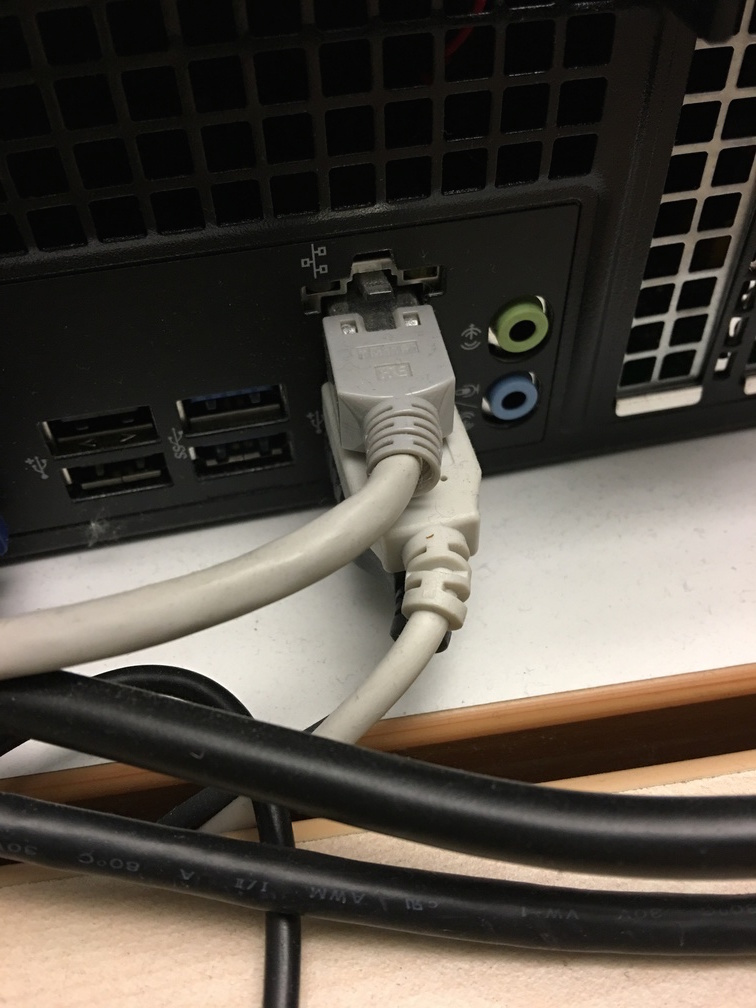
\includegraphics{igb/img/internet.jpg}
\end{center}

Zweifelsohne verbringen wir die meiste Zeit irgendwo im Netz. Wenn das
Netz ausfällt -- was es glücklicherweise selten macht --, merkt man das
erst richtig. Gut, dass es dann noch ein paar Bücherregale gibt, in
denen man mal wieder Ordnung schaffen kann.

\hypertarget{was-wuxfcrden-sie-vermissen-wenn-es-nicht-mehr-da-wuxe4re-wieso-wuxfcrden-sie-es-vermissen}{%
\subsubsection*{Was würden Sie vermissen, wenn es nicht mehr da wäre? Wieso
würden Sie es
vermissen?}\label{was-wuxfcrden-sie-vermissen-wenn-es-nicht-mehr-da-wuxe4re-wieso-wuxfcrden-sie-es-vermissen}}

\begin{center}
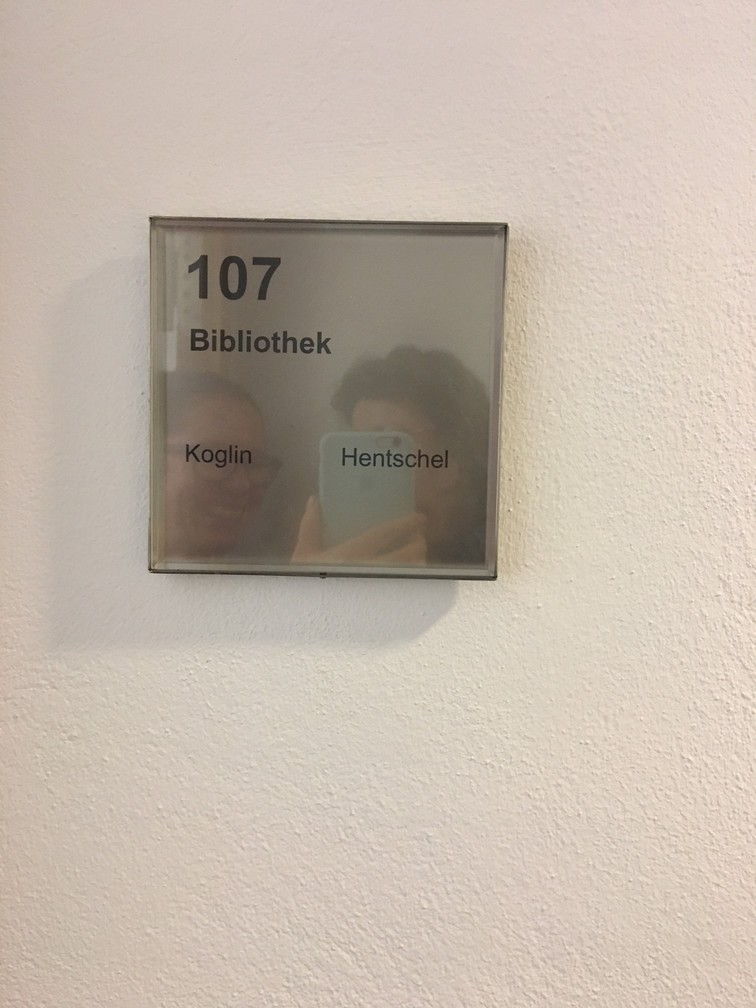
\includegraphics{igb/img/bibliothek.jpg}
\end{center}

Meine Kolleginnen. Wir sind eine Two-Persons-Library mit Hilfskraft und
ich habe einen sehr großen Respekt für Kolleginnen aus OPLs, die alles
alleine stemmen.

\hypertarget{was-stuxf6rt-sie-an-ihrer-bibliothek-beziehungsweise-was-wuxfcrden-sie-gerne-verbessern-wieso-stuxf6rt-sie-das-jetzt-noch}{%
\subsubsection*{Was stört Sie an Ihrer Bibliothek beziehungsweise was würden
Sie gerne verbessern? Wieso stört Sie das jetzt
(noch)?}\label{was-stuxf6rt-sie-an-ihrer-bibliothek-beziehungsweise-was-wuxfcrden-sie-gerne-verbessern-wieso-stuxf6rt-sie-das-jetzt-noch}}

\begin{center}
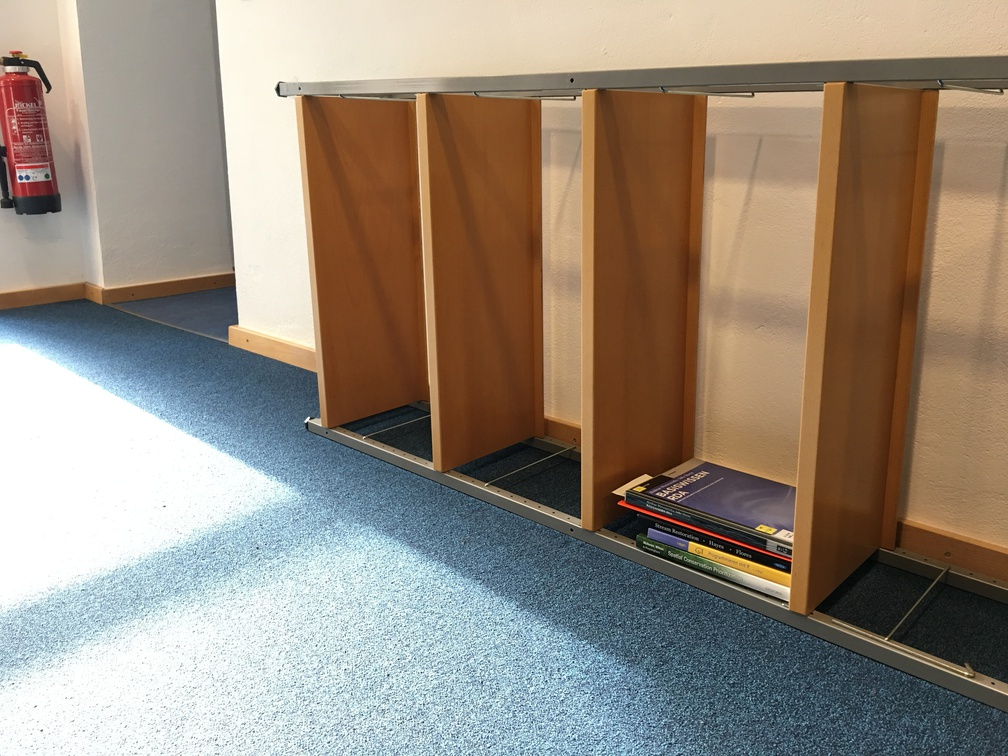
\includegraphics{igb/img/regal.jpg}
\end{center}

Wir sind gerade bei einem Projekt, bei dem wir mehrere tausend Bücher
umstellen. Physische Medien sind in ihrer Verwaltung, Bearbeitung und
täglichen Handhabung sehr aufwendig. Irgendwann dachte ich mal -- in den
Anfangsjahren der bibliothekarischen Tätigkeit -- so ein Regal ist
schnell umgeräumt oder ein paar Bücher schnell neu signiert. But, boy,
was I wrong\ldots{}

\hypertarget{zeigen-sie-uns-spuren-der-bibliotheksnutzung.-gibt-es-dazu-eine-geschichte}{%
\subsubsection*{Zeigen Sie uns Spuren der Bibliotheksnutzung. Gibt es dazu eine
Geschichte?}\label{zeigen-sie-uns-spuren-der-bibliotheksnutzung.-gibt-es-dazu-eine-geschichte}}

\begin{center}
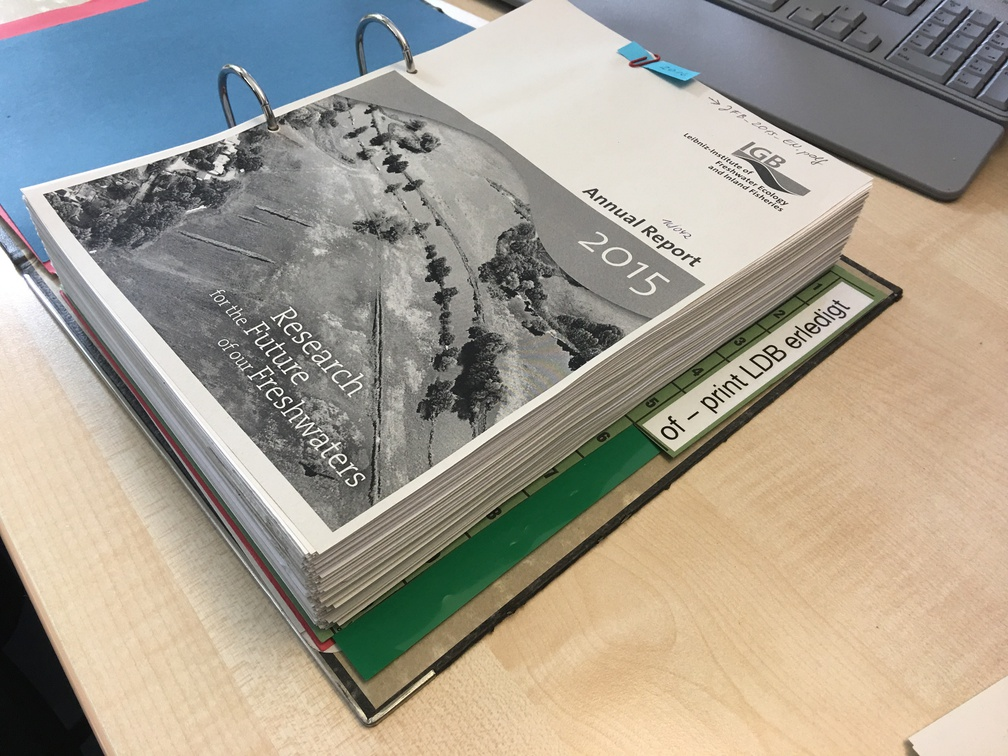
\includegraphics{igb/img/publikationen.jpg}
\end{center}

Auf dem Foto sieht man die ausgedruckten Titelseiten aller am Institut
erstellten Publikationen im Jahr 2016. Ich sehe sie auch als ein
Ergebnis der von Bibliotheken bereitgestellten gemeinsamen und lokalen
Infrastrukturen, ohne die Forschung nicht möglich wäre und die hier
wieder zurück in die Bibliothek finden.

\hypertarget{was-haben-sie-was-die-anderen-nicht-haben-warum-haben-sie-das-sollten-andere-es-auch-in-ihren-bibliotheken-haben}{%
\subsubsection*{Was haben Sie, was die anderen nicht haben? Warum haben Sie
das? Sollten andere es auch in ihren Bibliotheken
haben?}\label{was-haben-sie-was-die-anderen-nicht-haben-warum-haben-sie-das-sollten-andere-es-auch-in-ihren-bibliotheken-haben}}

\begin{center}
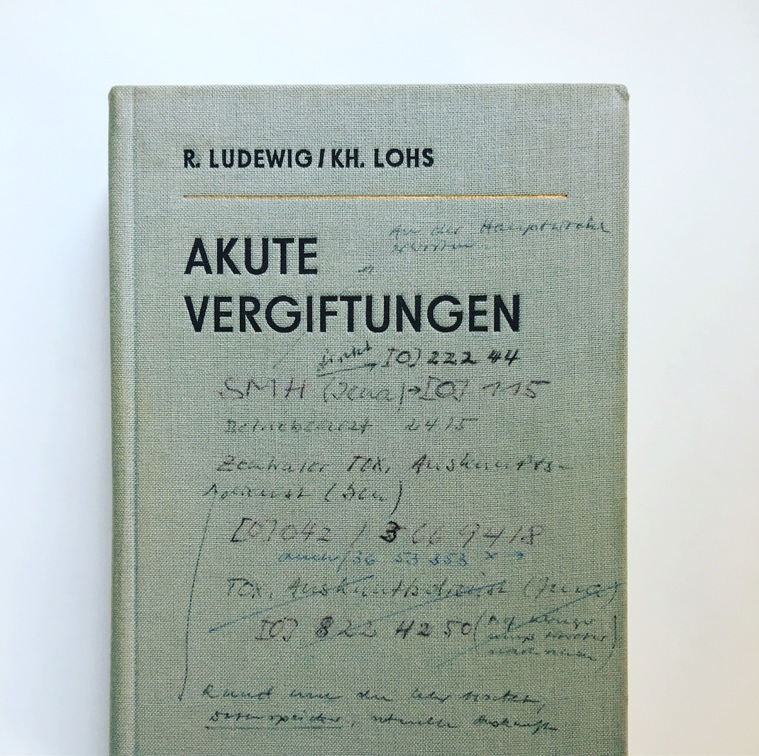
\includegraphics{igb/img/vergiftungen.jpg}
\end{center}

Auch wenn es das absolute No-Go ist, muss ich zugeben: Ich bin ein Fan
von Benutzungsspuren. Dieses Buch haben wir zufällig bei der
Bestandsdurchsicht gefunden. Elektronische Medien, für die wir heute den
Großteil unseres Budgets ausgeben, haben diese Spuren nicht. Bei allen
Vorteilen, die digitale Medien haben, vermisse ich es ein wenig, dass
Dateien niemals Geschichten erzählen werden können.

\hypertarget{ihre-bibliothek-name-adresse-spezialisierung-was-man-noch-uxfcber-sie-wissen-sollte}{%
\subsubsection*{Ihre Bibliothek (Name, Adresse, Spezialisierung, was man noch
über sie wissen
sollte)?}\label{ihre-bibliothek-name-adresse-spezialisierung-was-man-noch-uxfcber-sie-wissen-sollte}}

Bibliothek des Leibniz-Instituts für Gewässerökologie und
Binnenfischerei (IGB) im Forschungsverbund Berlin e.\,V., am Nordufer des
Müggelsees in Berlin-Friedrichshagen.

%autor
\begin{center}\rule{0.5\linewidth}{\linethickness}\end{center}

\textbf{Lydia Koglin}, nach geisteswissenschaftlichem Studium und
bibliothekswissenschaftlicher Ausbildung an einer Universitätsbibliothek
jetzt Leiterin einer Two-and-half-Woman-Bibliothek eines
umweltwissenschaftlichen Forschungsinstituts.
% !TEX root = ../master.tex

\vspace*{.5cm}
\section{Bibliothek des Leibniz-Instituts für Gewässerökologie und Binnenfischerei}
\begin{center}
\emph{Lydia Koglin}
\end{center}
\vspace*{1cm}

%body
\hypertarget{zeigen-sie-uns-den-ort-in-ihrer-bibliothek-an-dem-sie-die-meiste-zeit-verbringen.-was-ist-das-fuxfcr-ein-ort-wieso-sind-sie-die-meiste-zeit-dort}{%
\subsubsection*{Zeigen Sie uns den Ort in Ihrer Bibliothek, an dem Sie die
meiste Zeit verbringen. Was ist das für ein Ort? Wieso sind Sie die
meiste Zeit
dort?}\label{zeigen-sie-uns-den-ort-in-ihrer-bibliothek-an-dem-sie-die-meiste-zeit-verbringen.-was-ist-das-fuxfcr-ein-ort-wieso-sind-sie-die-meiste-zeit-dort}}

\begin{center}
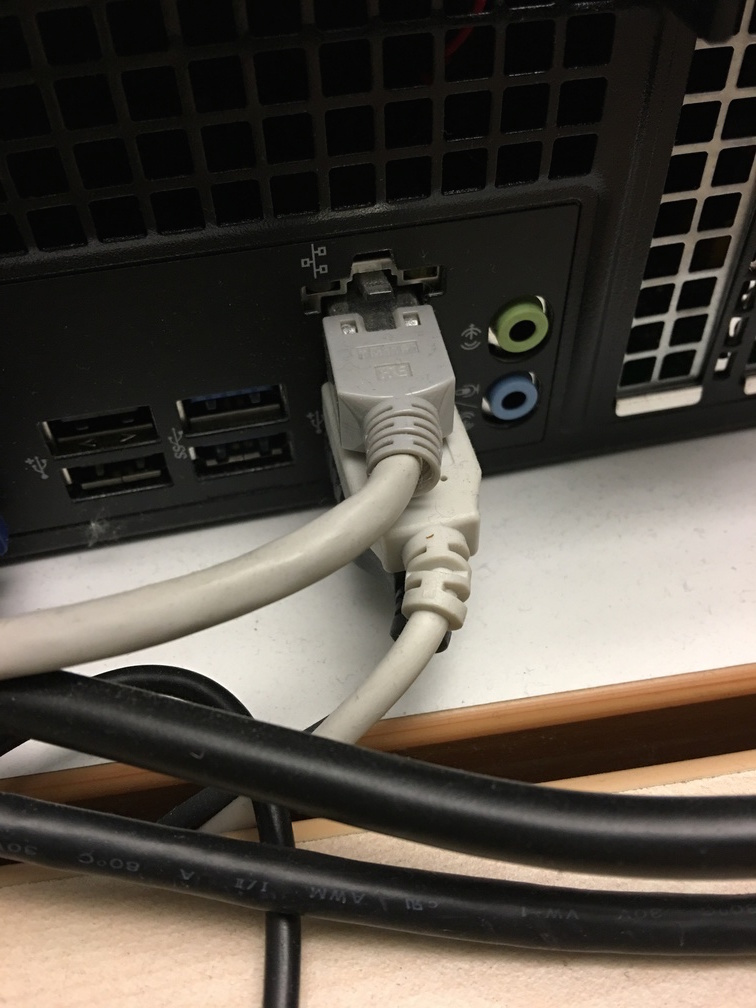
\includegraphics{igb/img/internet.jpg}
\end{center}

Zweifelsohne verbringen wir die meiste Zeit irgendwo im Netz. Wenn das
Netz ausfällt -- was es glücklicherweise selten macht --, merkt man das
erst richtig. Gut, dass es dann noch ein paar Bücherregale gibt, in
denen man mal wieder Ordnung schaffen kann.

\hypertarget{was-wuxfcrden-sie-vermissen-wenn-es-nicht-mehr-da-wuxe4re-wieso-wuxfcrden-sie-es-vermissen}{%
\subsubsection*{Was würden Sie vermissen, wenn es nicht mehr da wäre? Wieso
würden Sie es
vermissen?}\label{was-wuxfcrden-sie-vermissen-wenn-es-nicht-mehr-da-wuxe4re-wieso-wuxfcrden-sie-es-vermissen}}

\begin{center}
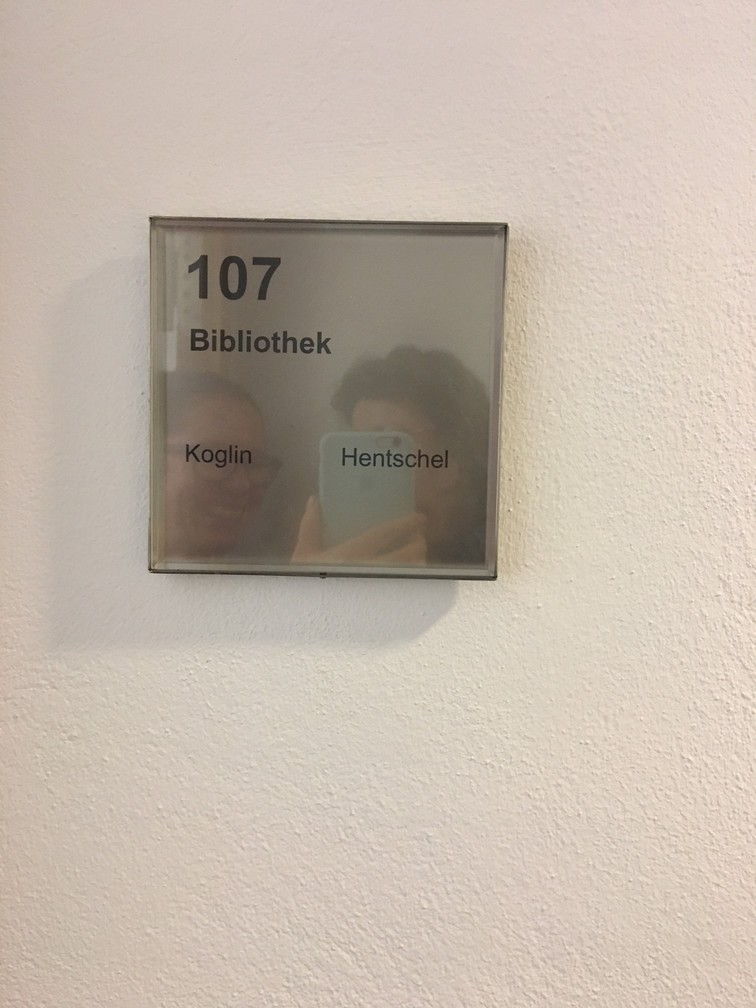
\includegraphics{igb/img/bibliothek.jpg}
\end{center}

Meine Kolleginnen. Wir sind eine Two-Persons-Library mit Hilfskraft und
ich habe einen sehr großen Respekt für Kolleginnen aus OPLs, die alles
alleine stemmen.

\hypertarget{was-stuxf6rt-sie-an-ihrer-bibliothek-beziehungsweise-was-wuxfcrden-sie-gerne-verbessern-wieso-stuxf6rt-sie-das-jetzt-noch}{%
\subsubsection*{Was stört Sie an Ihrer Bibliothek beziehungsweise was würden
Sie gerne verbessern? Wieso stört Sie das jetzt
(noch)?}\label{was-stuxf6rt-sie-an-ihrer-bibliothek-beziehungsweise-was-wuxfcrden-sie-gerne-verbessern-wieso-stuxf6rt-sie-das-jetzt-noch}}

\begin{center}
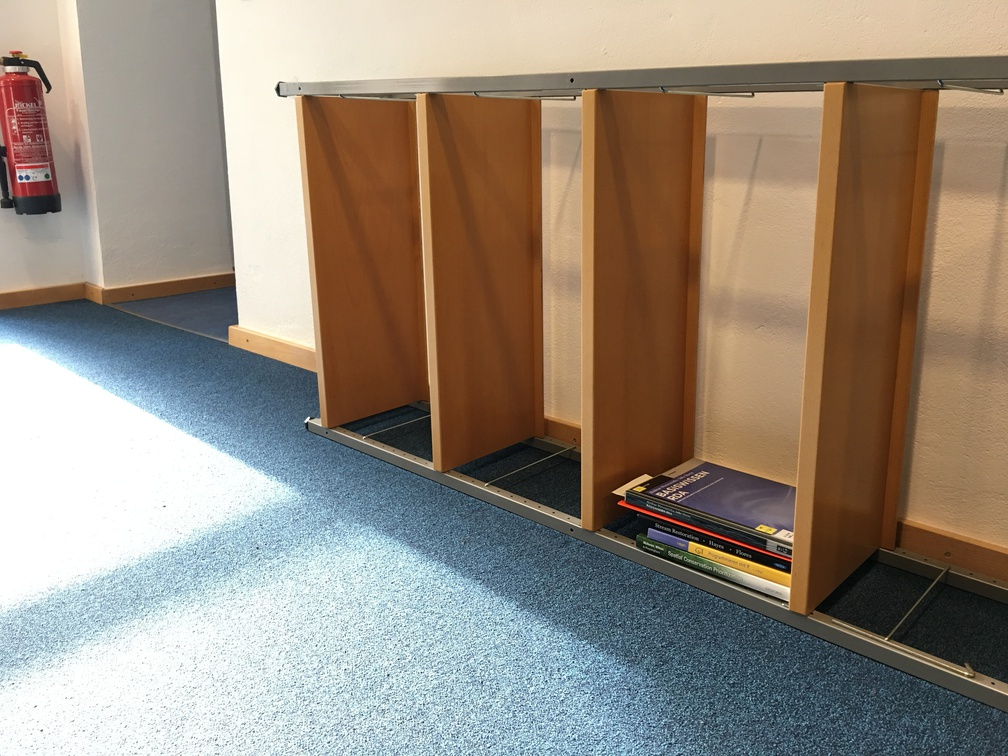
\includegraphics{igb/img/regal.jpg}
\end{center}

Wir sind gerade bei einem Projekt, bei dem wir mehrere tausend Bücher
umstellen. Physische Medien sind in ihrer Verwaltung, Bearbeitung und
täglichen Handhabung sehr aufwendig. Irgendwann dachte ich mal -- in den
Anfangsjahren der bibliothekarischen Tätigkeit -- so ein Regal ist
schnell umgeräumt oder ein paar Bücher schnell neu signiert. But, boy,
was I wrong\ldots{}

\hypertarget{zeigen-sie-uns-spuren-der-bibliotheksnutzung.-gibt-es-dazu-eine-geschichte}{%
\subsubsection*{Zeigen Sie uns Spuren der Bibliotheksnutzung. Gibt es dazu eine
Geschichte?}\label{zeigen-sie-uns-spuren-der-bibliotheksnutzung.-gibt-es-dazu-eine-geschichte}}

\begin{center}
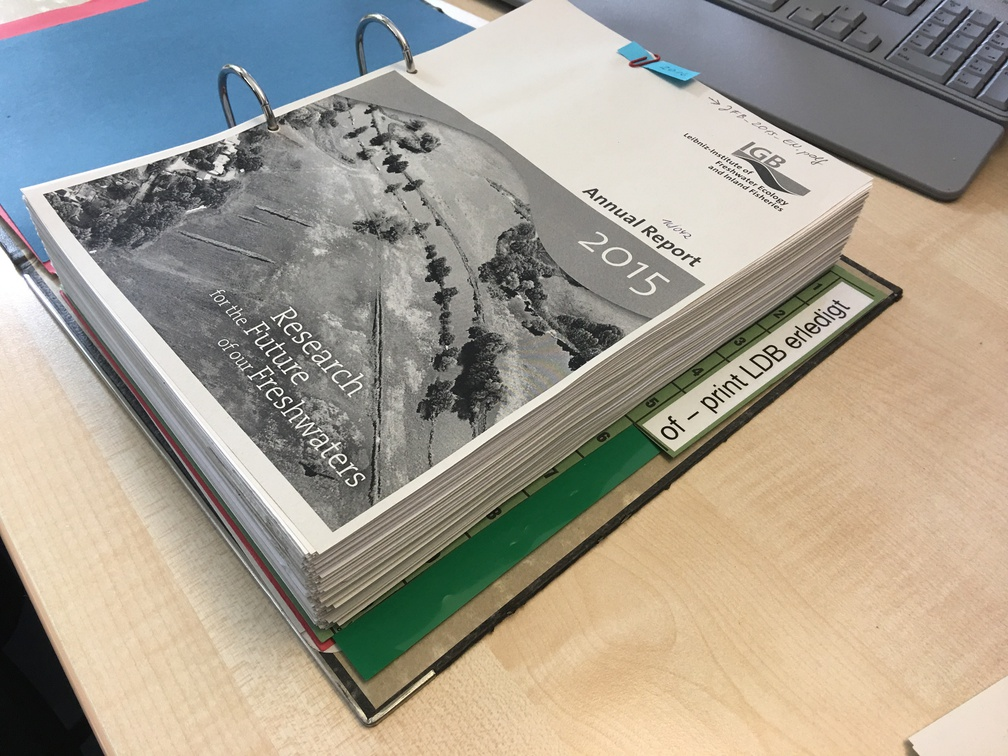
\includegraphics{igb/img/publikationen.jpg}
\end{center}

Auf dem Foto sieht man die ausgedruckten Titelseiten aller am Institut
erstellten Publikationen im Jahr 2016. Ich sehe sie auch als ein
Ergebnis der von Bibliotheken bereitgestellten gemeinsamen und lokalen
Infrastrukturen, ohne die Forschung nicht möglich wäre und die hier
wieder zurück in die Bibliothek finden.

\hypertarget{was-haben-sie-was-die-anderen-nicht-haben-warum-haben-sie-das-sollten-andere-es-auch-in-ihren-bibliotheken-haben}{%
\subsubsection*{Was haben Sie, was die anderen nicht haben? Warum haben Sie
das? Sollten andere es auch in ihren Bibliotheken
haben?}\label{was-haben-sie-was-die-anderen-nicht-haben-warum-haben-sie-das-sollten-andere-es-auch-in-ihren-bibliotheken-haben}}

\begin{center}
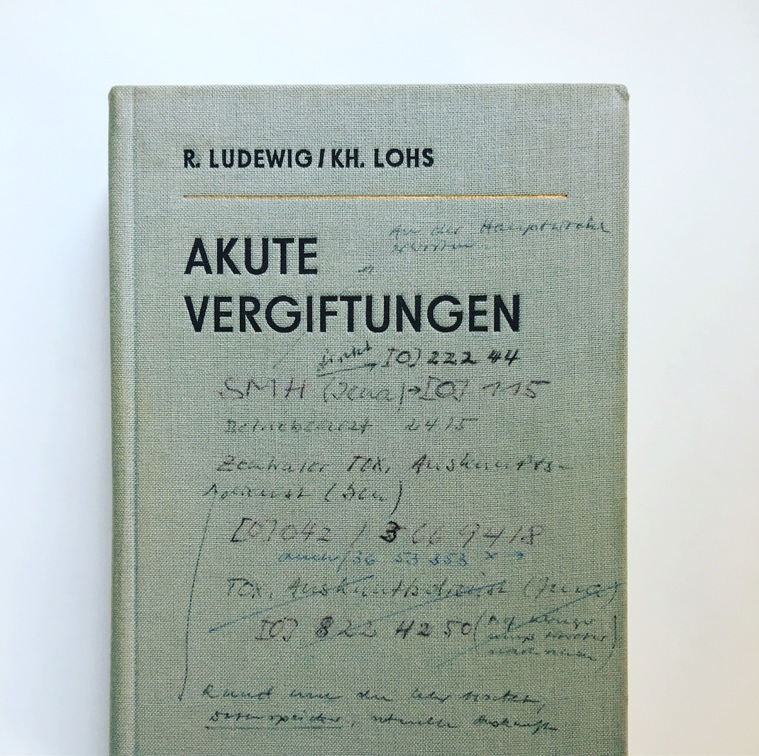
\includegraphics{igb/img/vergiftungen.jpg}
\end{center}

Auch wenn es das absolute No-Go ist, muss ich zugeben: Ich bin ein Fan
von Benutzungsspuren. Dieses Buch haben wir zufällig bei der
Bestandsdurchsicht gefunden. Elektronische Medien, für die wir heute den
Großteil unseres Budgets ausgeben, haben diese Spuren nicht. Bei allen
Vorteilen, die digitale Medien haben, vermisse ich es ein wenig, dass
Dateien niemals Geschichten erzählen werden können.

\hypertarget{ihre-bibliothek-name-adresse-spezialisierung-was-man-noch-uxfcber-sie-wissen-sollte}{%
\subsubsection*{Ihre Bibliothek (Name, Adresse, Spezialisierung, was man noch
über sie wissen
sollte)?}\label{ihre-bibliothek-name-adresse-spezialisierung-was-man-noch-uxfcber-sie-wissen-sollte}}

Bibliothek des Leibniz-Instituts für Gewässerökologie und
Binnenfischerei (IGB) im Forschungsverbund Berlin e.\,V., am Nordufer des
Müggelsees in Berlin-Friedrichshagen.

%autor
\begin{center}\rule{0.5\linewidth}{\linethickness}\end{center}

\textbf{Lydia Koglin}, nach geisteswissenschaftlichem Studium und
bibliothekswissenschaftlicher Ausbildung an einer Universitätsbibliothek
jetzt Leiterin einer Two-and-half-Woman-Bibliothek eines
umweltwissenschaftlichen Forschungsinstituts.
% !TEX root = ../master.tex

\vspace*{.5cm}
\section{Bibliothek des Leibniz-Instituts für Gewässerökologie und Binnenfischerei}
\begin{center}
\emph{Lydia Koglin}
\end{center}
\vspace*{1cm}

%body
\hypertarget{zeigen-sie-uns-den-ort-in-ihrer-bibliothek-an-dem-sie-die-meiste-zeit-verbringen.-was-ist-das-fuxfcr-ein-ort-wieso-sind-sie-die-meiste-zeit-dort}{%
\subsubsection*{Zeigen Sie uns den Ort in Ihrer Bibliothek, an dem Sie die
meiste Zeit verbringen. Was ist das für ein Ort? Wieso sind Sie die
meiste Zeit
dort?}\label{zeigen-sie-uns-den-ort-in-ihrer-bibliothek-an-dem-sie-die-meiste-zeit-verbringen.-was-ist-das-fuxfcr-ein-ort-wieso-sind-sie-die-meiste-zeit-dort}}

\begin{center}
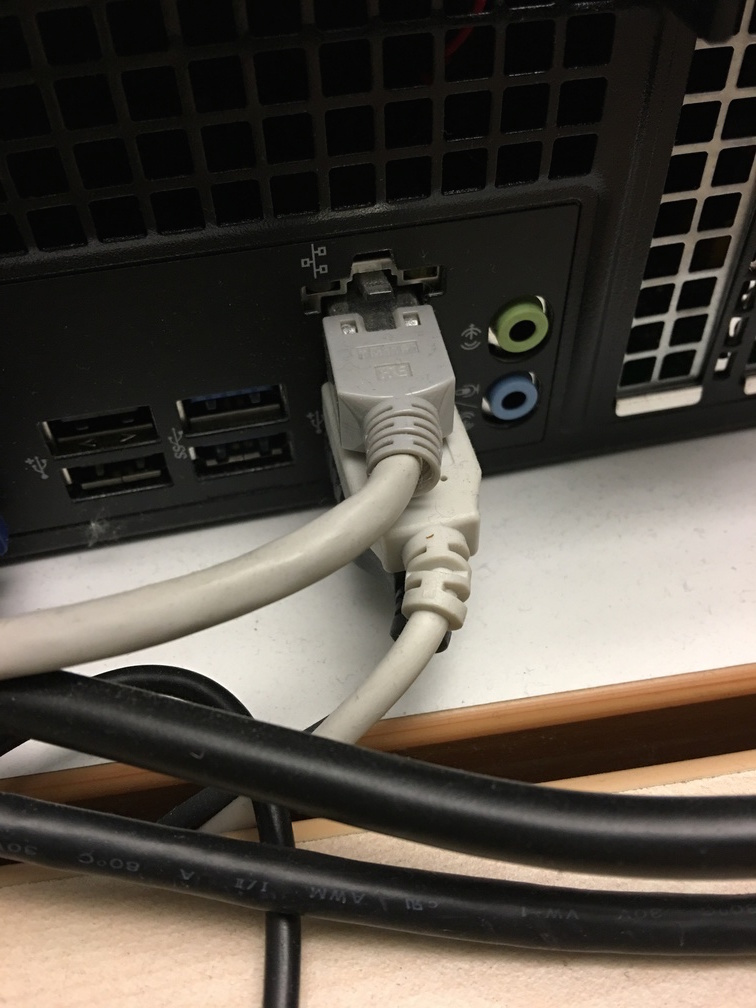
\includegraphics{igb/img/internet.jpg}
\end{center}

Zweifelsohne verbringen wir die meiste Zeit irgendwo im Netz. Wenn das
Netz ausfällt -- was es glücklicherweise selten macht --, merkt man das
erst richtig. Gut, dass es dann noch ein paar Bücherregale gibt, in
denen man mal wieder Ordnung schaffen kann.

\hypertarget{was-wuxfcrden-sie-vermissen-wenn-es-nicht-mehr-da-wuxe4re-wieso-wuxfcrden-sie-es-vermissen}{%
\subsubsection*{Was würden Sie vermissen, wenn es nicht mehr da wäre? Wieso
würden Sie es
vermissen?}\label{was-wuxfcrden-sie-vermissen-wenn-es-nicht-mehr-da-wuxe4re-wieso-wuxfcrden-sie-es-vermissen}}

\begin{center}
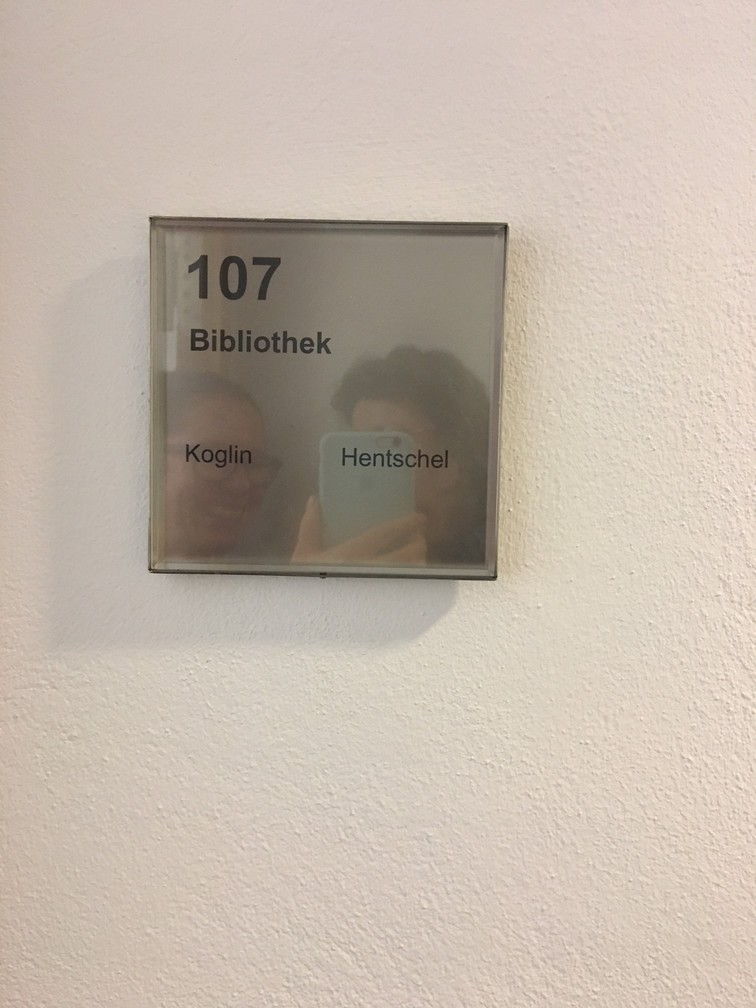
\includegraphics{igb/img/bibliothek.jpg}
\end{center}

Meine Kolleginnen. Wir sind eine Two-Persons-Library mit Hilfskraft und
ich habe einen sehr großen Respekt für Kolleginnen aus OPLs, die alles
alleine stemmen.

\hypertarget{was-stuxf6rt-sie-an-ihrer-bibliothek-beziehungsweise-was-wuxfcrden-sie-gerne-verbessern-wieso-stuxf6rt-sie-das-jetzt-noch}{%
\subsubsection*{Was stört Sie an Ihrer Bibliothek beziehungsweise was würden
Sie gerne verbessern? Wieso stört Sie das jetzt
(noch)?}\label{was-stuxf6rt-sie-an-ihrer-bibliothek-beziehungsweise-was-wuxfcrden-sie-gerne-verbessern-wieso-stuxf6rt-sie-das-jetzt-noch}}

\begin{center}
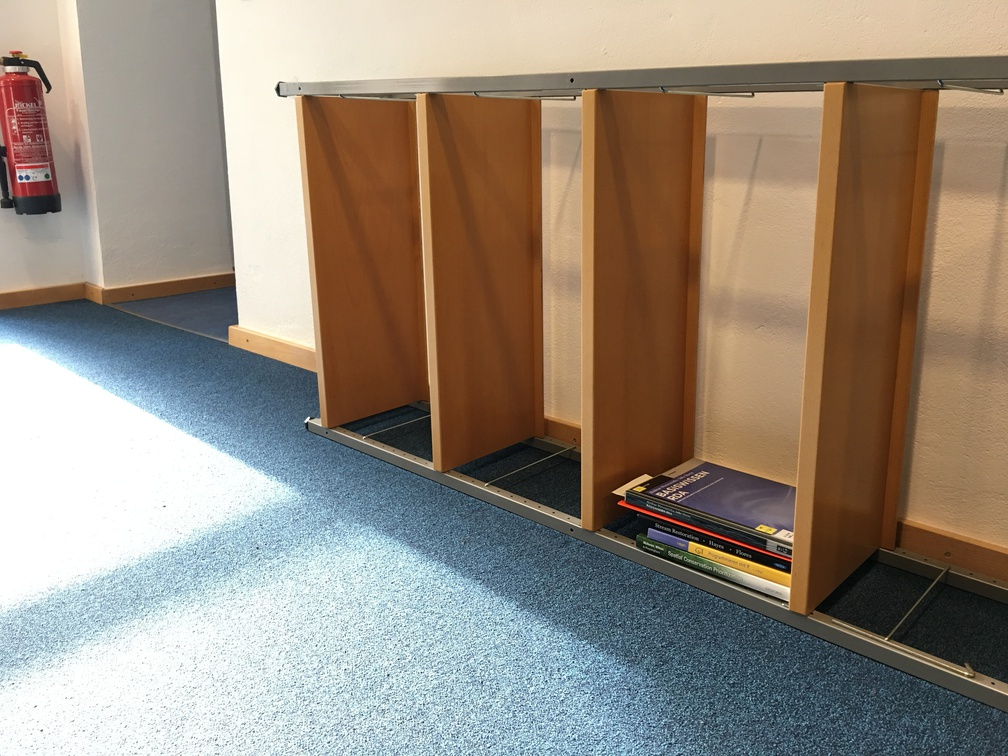
\includegraphics{igb/img/regal.jpg}
\end{center}

Wir sind gerade bei einem Projekt, bei dem wir mehrere tausend Bücher
umstellen. Physische Medien sind in ihrer Verwaltung, Bearbeitung und
täglichen Handhabung sehr aufwendig. Irgendwann dachte ich mal -- in den
Anfangsjahren der bibliothekarischen Tätigkeit -- so ein Regal ist
schnell umgeräumt oder ein paar Bücher schnell neu signiert. But, boy,
was I wrong\ldots{}

\hypertarget{zeigen-sie-uns-spuren-der-bibliotheksnutzung.-gibt-es-dazu-eine-geschichte}{%
\subsubsection*{Zeigen Sie uns Spuren der Bibliotheksnutzung. Gibt es dazu eine
Geschichte?}\label{zeigen-sie-uns-spuren-der-bibliotheksnutzung.-gibt-es-dazu-eine-geschichte}}

\begin{center}
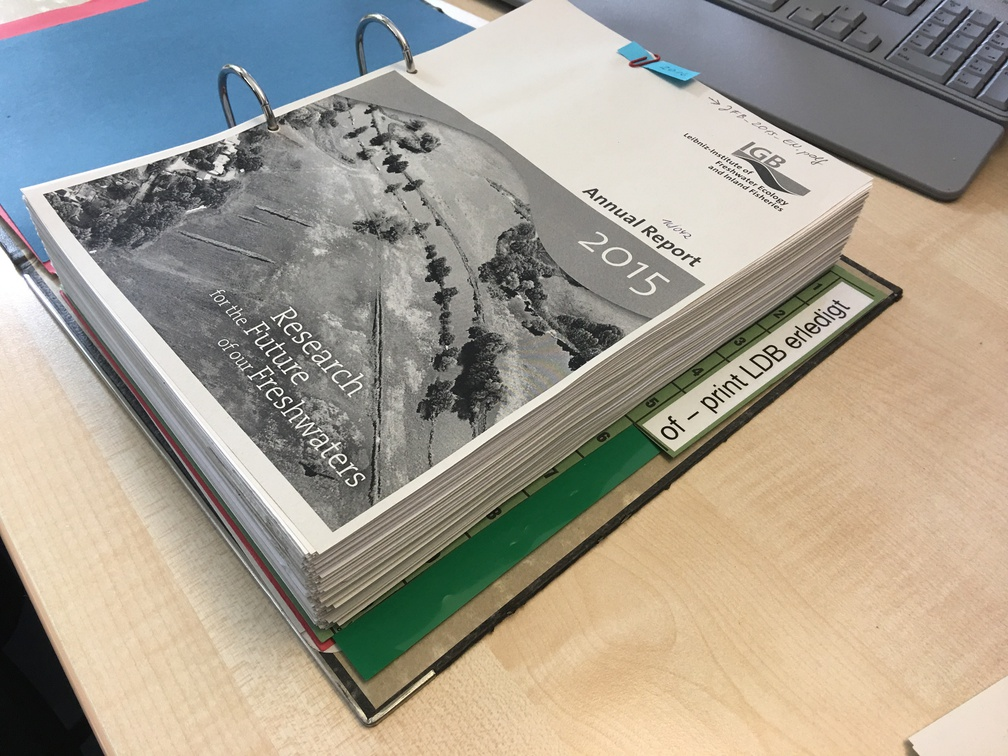
\includegraphics{igb/img/publikationen.jpg}
\end{center}

Auf dem Foto sieht man die ausgedruckten Titelseiten aller am Institut
erstellten Publikationen im Jahr 2016. Ich sehe sie auch als ein
Ergebnis der von Bibliotheken bereitgestellten gemeinsamen und lokalen
Infrastrukturen, ohne die Forschung nicht möglich wäre und die hier
wieder zurück in die Bibliothek finden.

\hypertarget{was-haben-sie-was-die-anderen-nicht-haben-warum-haben-sie-das-sollten-andere-es-auch-in-ihren-bibliotheken-haben}{%
\subsubsection*{Was haben Sie, was die anderen nicht haben? Warum haben Sie
das? Sollten andere es auch in ihren Bibliotheken
haben?}\label{was-haben-sie-was-die-anderen-nicht-haben-warum-haben-sie-das-sollten-andere-es-auch-in-ihren-bibliotheken-haben}}

\begin{center}
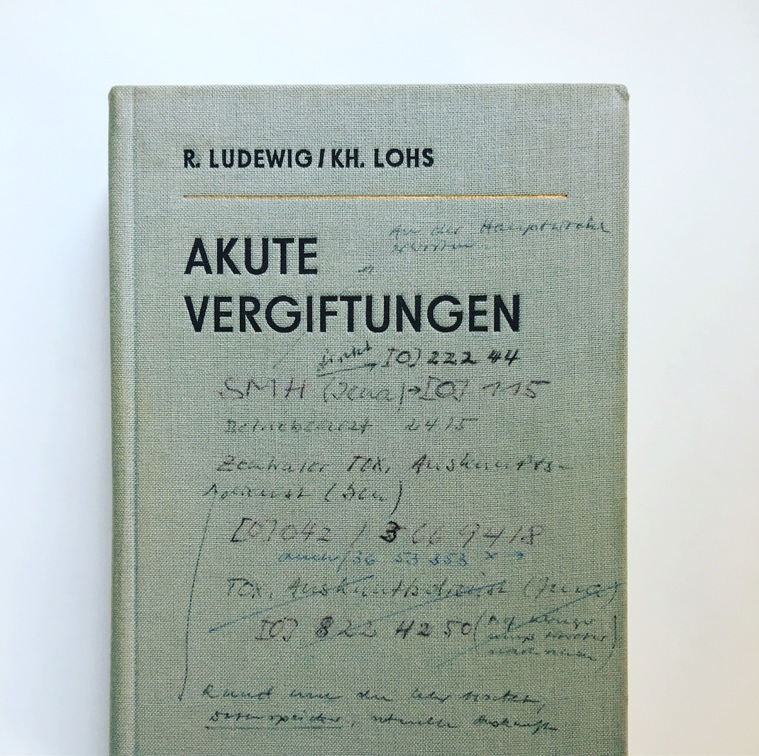
\includegraphics{igb/img/vergiftungen.jpg}
\end{center}

Auch wenn es das absolute No-Go ist, muss ich zugeben: Ich bin ein Fan
von Benutzungsspuren. Dieses Buch haben wir zufällig bei der
Bestandsdurchsicht gefunden. Elektronische Medien, für die wir heute den
Großteil unseres Budgets ausgeben, haben diese Spuren nicht. Bei allen
Vorteilen, die digitale Medien haben, vermisse ich es ein wenig, dass
Dateien niemals Geschichten erzählen werden können.

\hypertarget{ihre-bibliothek-name-adresse-spezialisierung-was-man-noch-uxfcber-sie-wissen-sollte}{%
\subsubsection*{Ihre Bibliothek (Name, Adresse, Spezialisierung, was man noch
über sie wissen
sollte)?}\label{ihre-bibliothek-name-adresse-spezialisierung-was-man-noch-uxfcber-sie-wissen-sollte}}

Bibliothek des Leibniz-Instituts für Gewässerökologie und
Binnenfischerei (IGB) im Forschungsverbund Berlin e.\,V., am Nordufer des
Müggelsees in Berlin-Friedrichshagen.

%autor
\begin{center}\rule{0.5\linewidth}{\linethickness}\end{center}

\textbf{Lydia Koglin}, nach geisteswissenschaftlichem Studium und
bibliothekswissenschaftlicher Ausbildung an einer Universitätsbibliothek
jetzt Leiterin einer Two-and-half-Woman-Bibliothek eines
umweltwissenschaftlichen Forschungsinstituts.
% !TEX root = ../master.tex

\vspace*{.5cm}
\section{Bibliothek des Leibniz-Instituts für Gewässerökologie und Binnenfischerei}
\begin{center}
\emph{Lydia Koglin}
\end{center}
\vspace*{1cm}

%body
\hypertarget{zeigen-sie-uns-den-ort-in-ihrer-bibliothek-an-dem-sie-die-meiste-zeit-verbringen.-was-ist-das-fuxfcr-ein-ort-wieso-sind-sie-die-meiste-zeit-dort}{%
\subsubsection*{Zeigen Sie uns den Ort in Ihrer Bibliothek, an dem Sie die
meiste Zeit verbringen. Was ist das für ein Ort? Wieso sind Sie die
meiste Zeit
dort?}\label{zeigen-sie-uns-den-ort-in-ihrer-bibliothek-an-dem-sie-die-meiste-zeit-verbringen.-was-ist-das-fuxfcr-ein-ort-wieso-sind-sie-die-meiste-zeit-dort}}

\begin{center}
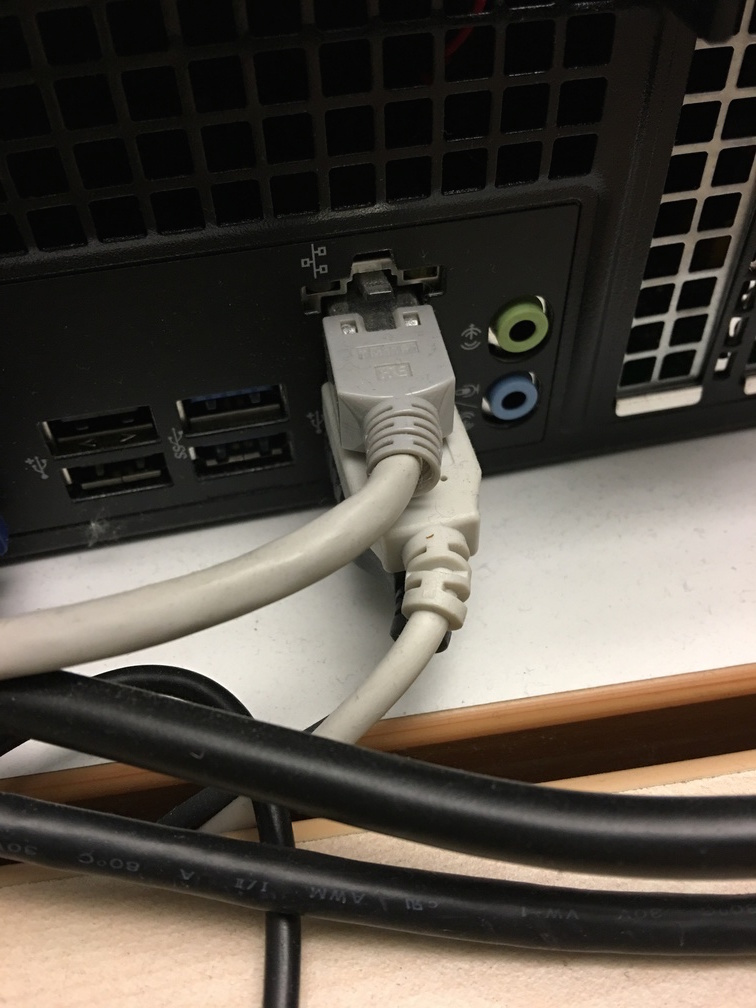
\includegraphics{igb/img/internet.jpg}
\end{center}

Zweifelsohne verbringen wir die meiste Zeit irgendwo im Netz. Wenn das
Netz ausfällt -- was es glücklicherweise selten macht --, merkt man das
erst richtig. Gut, dass es dann noch ein paar Bücherregale gibt, in
denen man mal wieder Ordnung schaffen kann.

\hypertarget{was-wuxfcrden-sie-vermissen-wenn-es-nicht-mehr-da-wuxe4re-wieso-wuxfcrden-sie-es-vermissen}{%
\subsubsection*{Was würden Sie vermissen, wenn es nicht mehr da wäre? Wieso
würden Sie es
vermissen?}\label{was-wuxfcrden-sie-vermissen-wenn-es-nicht-mehr-da-wuxe4re-wieso-wuxfcrden-sie-es-vermissen}}

\begin{center}
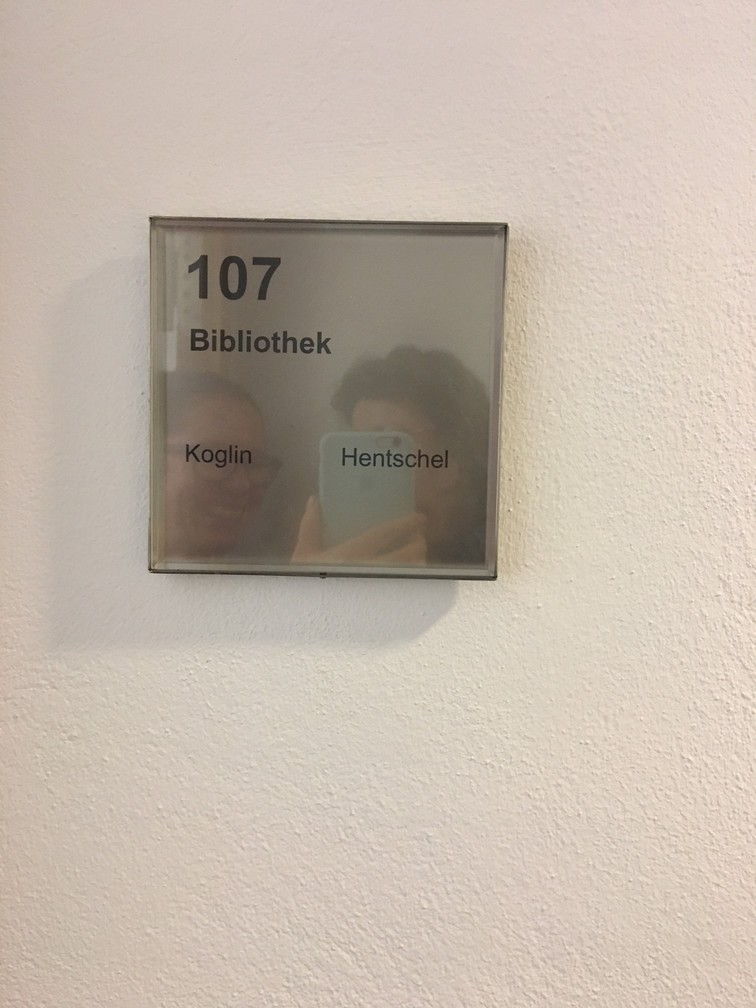
\includegraphics{igb/img/bibliothek.jpg}
\end{center}

Meine Kolleginnen. Wir sind eine Two-Persons-Library mit Hilfskraft und
ich habe einen sehr großen Respekt für Kolleginnen aus OPLs, die alles
alleine stemmen.

\hypertarget{was-stuxf6rt-sie-an-ihrer-bibliothek-beziehungsweise-was-wuxfcrden-sie-gerne-verbessern-wieso-stuxf6rt-sie-das-jetzt-noch}{%
\subsubsection*{Was stört Sie an Ihrer Bibliothek beziehungsweise was würden
Sie gerne verbessern? Wieso stört Sie das jetzt
(noch)?}\label{was-stuxf6rt-sie-an-ihrer-bibliothek-beziehungsweise-was-wuxfcrden-sie-gerne-verbessern-wieso-stuxf6rt-sie-das-jetzt-noch}}

\begin{center}
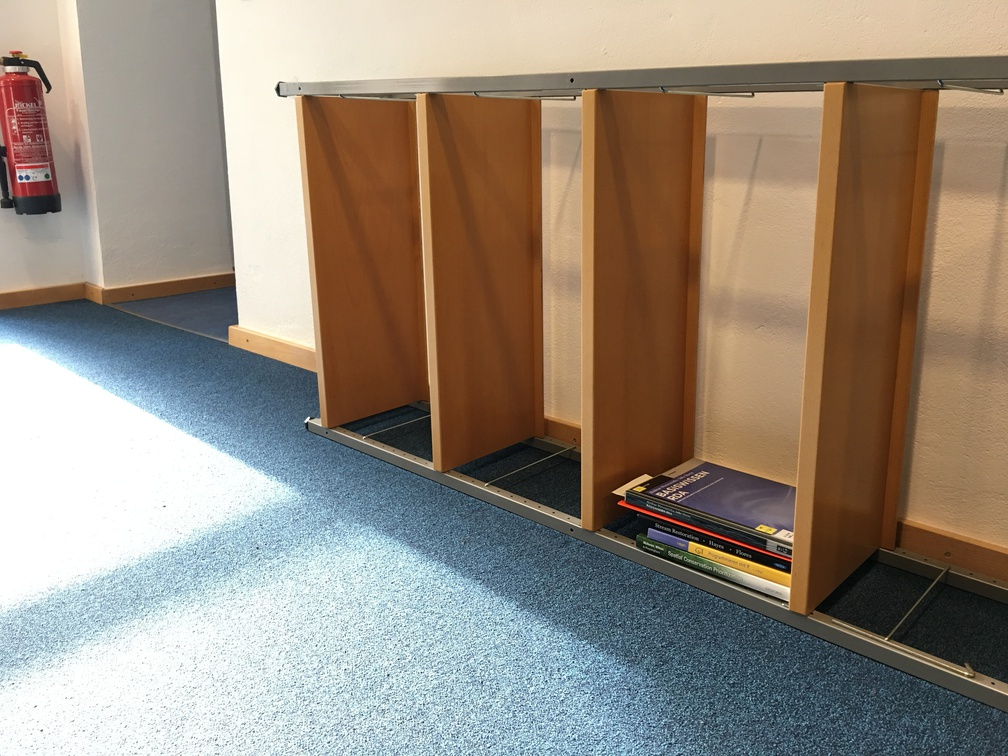
\includegraphics{igb/img/regal.jpg}
\end{center}

Wir sind gerade bei einem Projekt, bei dem wir mehrere tausend Bücher
umstellen. Physische Medien sind in ihrer Verwaltung, Bearbeitung und
täglichen Handhabung sehr aufwendig. Irgendwann dachte ich mal -- in den
Anfangsjahren der bibliothekarischen Tätigkeit -- so ein Regal ist
schnell umgeräumt oder ein paar Bücher schnell neu signiert. But, boy,
was I wrong\ldots{}

\hypertarget{zeigen-sie-uns-spuren-der-bibliotheksnutzung.-gibt-es-dazu-eine-geschichte}{%
\subsubsection*{Zeigen Sie uns Spuren der Bibliotheksnutzung. Gibt es dazu eine
Geschichte?}\label{zeigen-sie-uns-spuren-der-bibliotheksnutzung.-gibt-es-dazu-eine-geschichte}}

\begin{center}
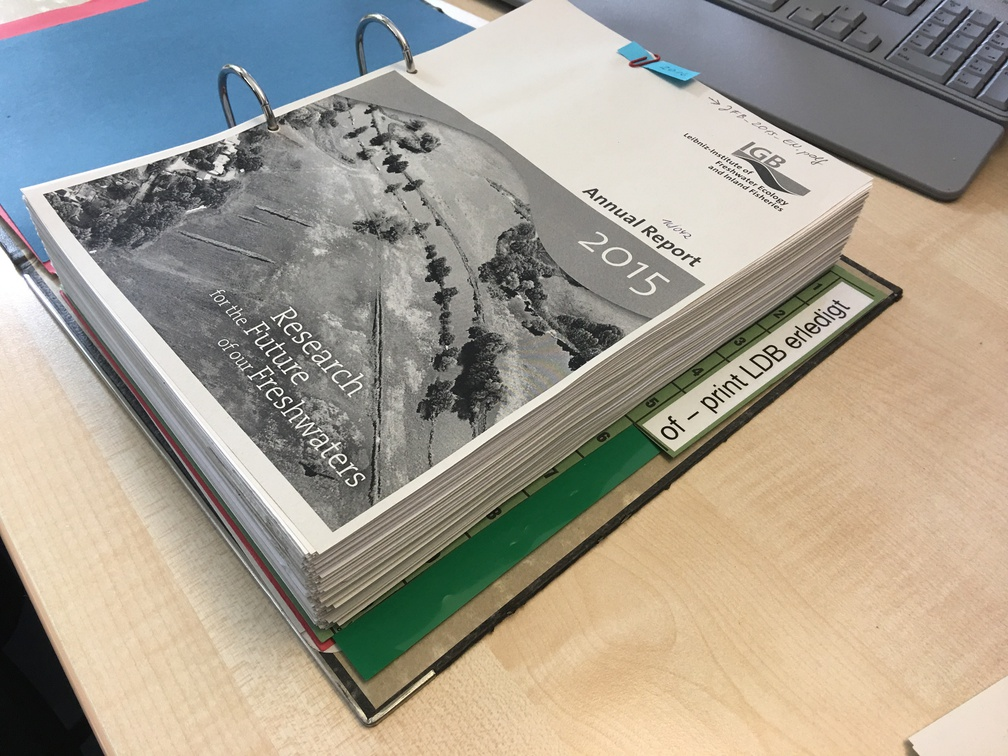
\includegraphics{igb/img/publikationen.jpg}
\end{center}

Auf dem Foto sieht man die ausgedruckten Titelseiten aller am Institut
erstellten Publikationen im Jahr 2016. Ich sehe sie auch als ein
Ergebnis der von Bibliotheken bereitgestellten gemeinsamen und lokalen
Infrastrukturen, ohne die Forschung nicht möglich wäre und die hier
wieder zurück in die Bibliothek finden.

\hypertarget{was-haben-sie-was-die-anderen-nicht-haben-warum-haben-sie-das-sollten-andere-es-auch-in-ihren-bibliotheken-haben}{%
\subsubsection*{Was haben Sie, was die anderen nicht haben? Warum haben Sie
das? Sollten andere es auch in ihren Bibliotheken
haben?}\label{was-haben-sie-was-die-anderen-nicht-haben-warum-haben-sie-das-sollten-andere-es-auch-in-ihren-bibliotheken-haben}}

\begin{center}
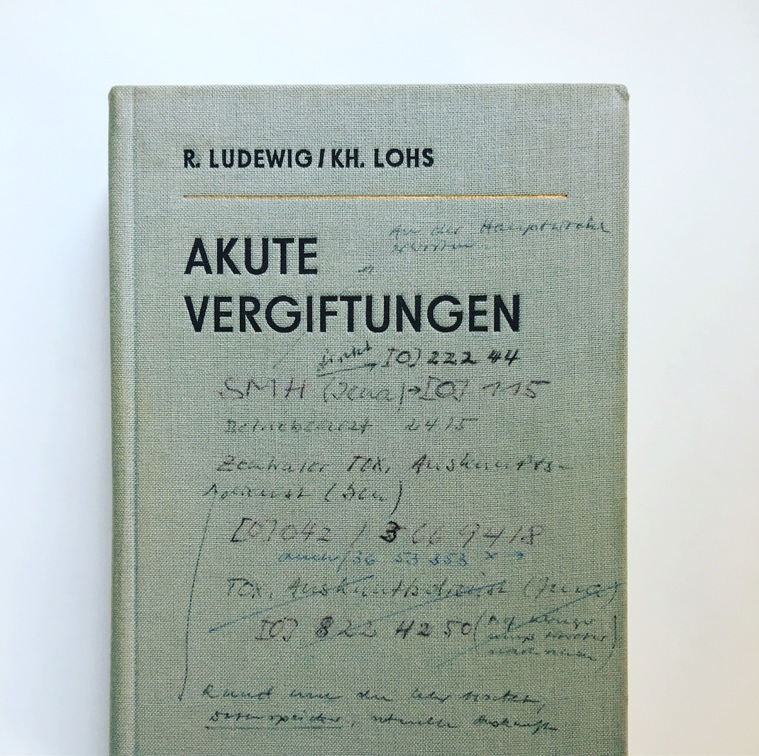
\includegraphics{igb/img/vergiftungen.jpg}
\end{center}

Auch wenn es das absolute No-Go ist, muss ich zugeben: Ich bin ein Fan
von Benutzungsspuren. Dieses Buch haben wir zufällig bei der
Bestandsdurchsicht gefunden. Elektronische Medien, für die wir heute den
Großteil unseres Budgets ausgeben, haben diese Spuren nicht. Bei allen
Vorteilen, die digitale Medien haben, vermisse ich es ein wenig, dass
Dateien niemals Geschichten erzählen werden können.

\hypertarget{ihre-bibliothek-name-adresse-spezialisierung-was-man-noch-uxfcber-sie-wissen-sollte}{%
\subsubsection*{Ihre Bibliothek (Name, Adresse, Spezialisierung, was man noch
über sie wissen
sollte)?}\label{ihre-bibliothek-name-adresse-spezialisierung-was-man-noch-uxfcber-sie-wissen-sollte}}

Bibliothek des Leibniz-Instituts für Gewässerökologie und
Binnenfischerei (IGB) im Forschungsverbund Berlin e.\,V., am Nordufer des
Müggelsees in Berlin-Friedrichshagen.

%autor
\begin{center}\rule{0.5\linewidth}{\linethickness}\end{center}

\textbf{Lydia Koglin}, nach geisteswissenschaftlichem Studium und
bibliothekswissenschaftlicher Ausbildung an einer Universitätsbibliothek
jetzt Leiterin einer Two-and-half-Woman-Bibliothek eines
umweltwissenschaftlichen Forschungsinstituts.
% !TEX root = ../master.tex

\vspace*{.5cm}
\section{Bibliothek des Leibniz-Instituts für Gewässerökologie und Binnenfischerei}
\begin{center}
\emph{Lydia Koglin}
\end{center}
\vspace*{1cm}

%body
\hypertarget{zeigen-sie-uns-den-ort-in-ihrer-bibliothek-an-dem-sie-die-meiste-zeit-verbringen.-was-ist-das-fuxfcr-ein-ort-wieso-sind-sie-die-meiste-zeit-dort}{%
\subsubsection*{Zeigen Sie uns den Ort in Ihrer Bibliothek, an dem Sie die
meiste Zeit verbringen. Was ist das für ein Ort? Wieso sind Sie die
meiste Zeit
dort?}\label{zeigen-sie-uns-den-ort-in-ihrer-bibliothek-an-dem-sie-die-meiste-zeit-verbringen.-was-ist-das-fuxfcr-ein-ort-wieso-sind-sie-die-meiste-zeit-dort}}

\begin{center}
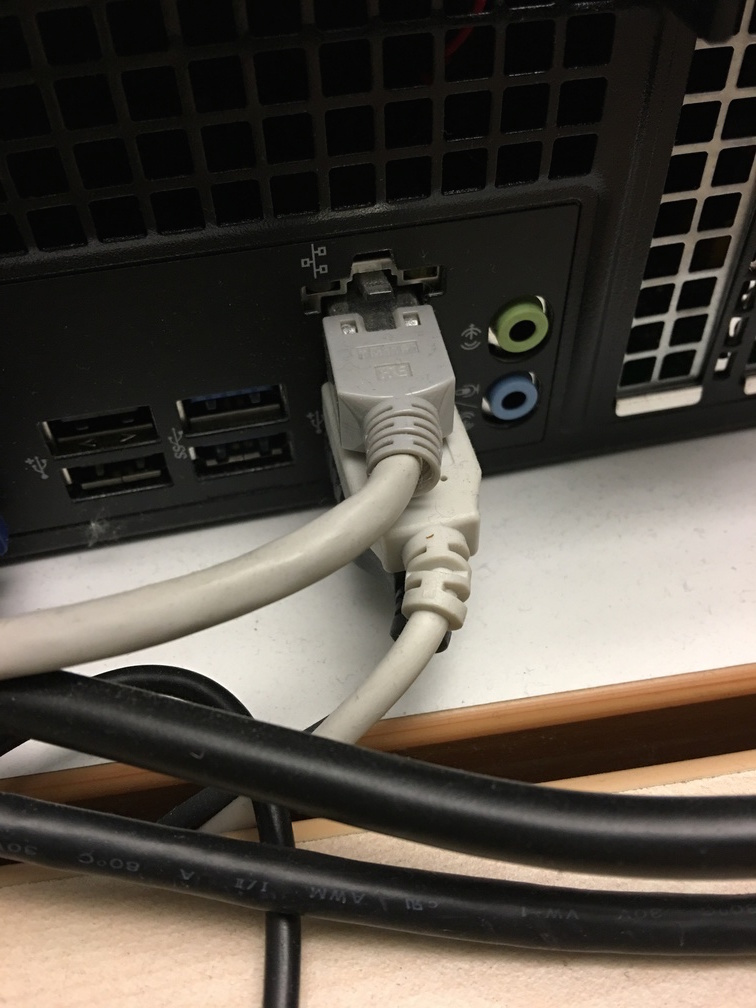
\includegraphics{igb/img/internet.jpg}
\end{center}

Zweifelsohne verbringen wir die meiste Zeit irgendwo im Netz. Wenn das
Netz ausfällt -- was es glücklicherweise selten macht --, merkt man das
erst richtig. Gut, dass es dann noch ein paar Bücherregale gibt, in
denen man mal wieder Ordnung schaffen kann.

\hypertarget{was-wuxfcrden-sie-vermissen-wenn-es-nicht-mehr-da-wuxe4re-wieso-wuxfcrden-sie-es-vermissen}{%
\subsubsection*{Was würden Sie vermissen, wenn es nicht mehr da wäre? Wieso
würden Sie es
vermissen?}\label{was-wuxfcrden-sie-vermissen-wenn-es-nicht-mehr-da-wuxe4re-wieso-wuxfcrden-sie-es-vermissen}}

\begin{center}
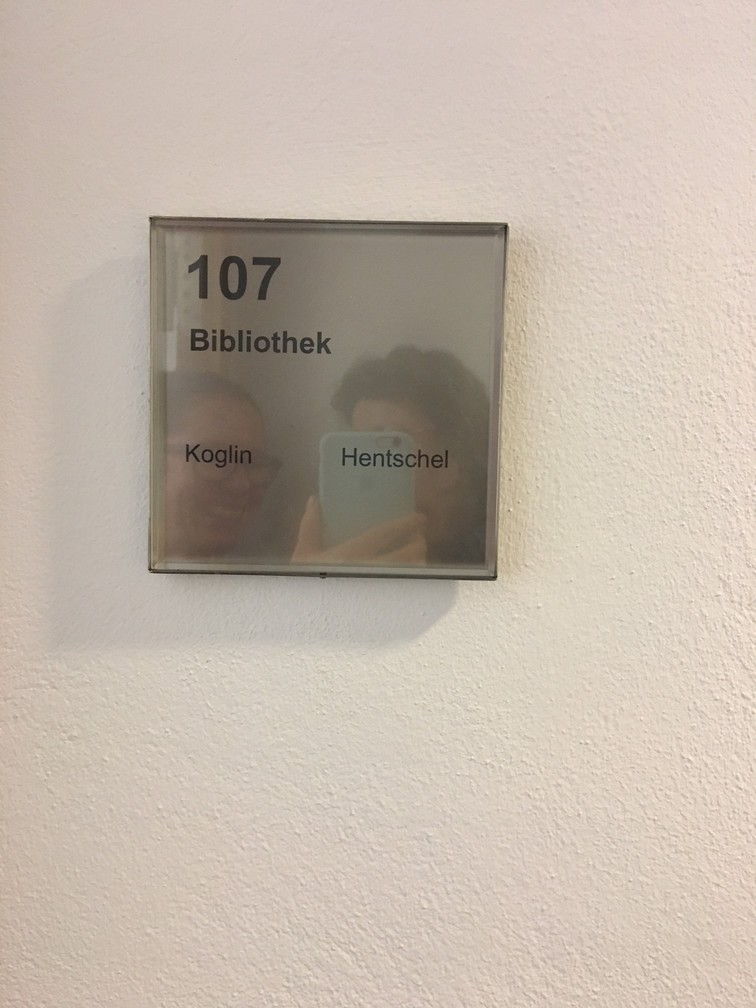
\includegraphics{igb/img/bibliothek.jpg}
\end{center}

Meine Kolleginnen. Wir sind eine Two-Persons-Library mit Hilfskraft und
ich habe einen sehr großen Respekt für Kolleginnen aus OPLs, die alles
alleine stemmen.

\hypertarget{was-stuxf6rt-sie-an-ihrer-bibliothek-beziehungsweise-was-wuxfcrden-sie-gerne-verbessern-wieso-stuxf6rt-sie-das-jetzt-noch}{%
\subsubsection*{Was stört Sie an Ihrer Bibliothek beziehungsweise was würden
Sie gerne verbessern? Wieso stört Sie das jetzt
(noch)?}\label{was-stuxf6rt-sie-an-ihrer-bibliothek-beziehungsweise-was-wuxfcrden-sie-gerne-verbessern-wieso-stuxf6rt-sie-das-jetzt-noch}}

\begin{center}
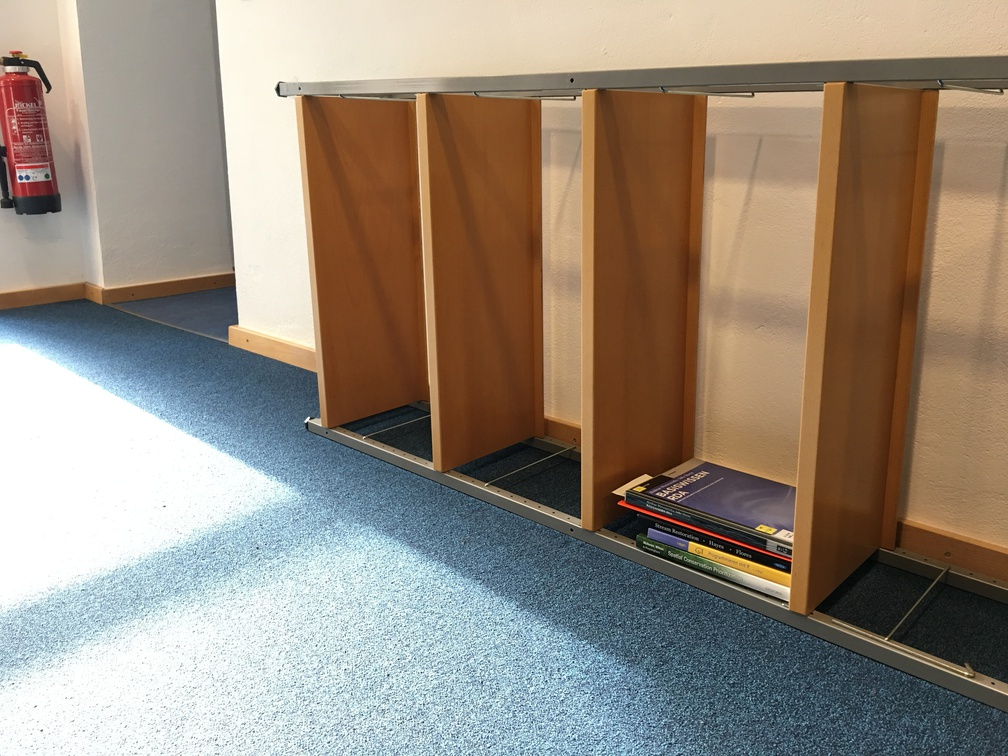
\includegraphics{igb/img/regal.jpg}
\end{center}

Wir sind gerade bei einem Projekt, bei dem wir mehrere tausend Bücher
umstellen. Physische Medien sind in ihrer Verwaltung, Bearbeitung und
täglichen Handhabung sehr aufwendig. Irgendwann dachte ich mal -- in den
Anfangsjahren der bibliothekarischen Tätigkeit -- so ein Regal ist
schnell umgeräumt oder ein paar Bücher schnell neu signiert. But, boy,
was I wrong\ldots{}

\hypertarget{zeigen-sie-uns-spuren-der-bibliotheksnutzung.-gibt-es-dazu-eine-geschichte}{%
\subsubsection*{Zeigen Sie uns Spuren der Bibliotheksnutzung. Gibt es dazu eine
Geschichte?}\label{zeigen-sie-uns-spuren-der-bibliotheksnutzung.-gibt-es-dazu-eine-geschichte}}

\begin{center}
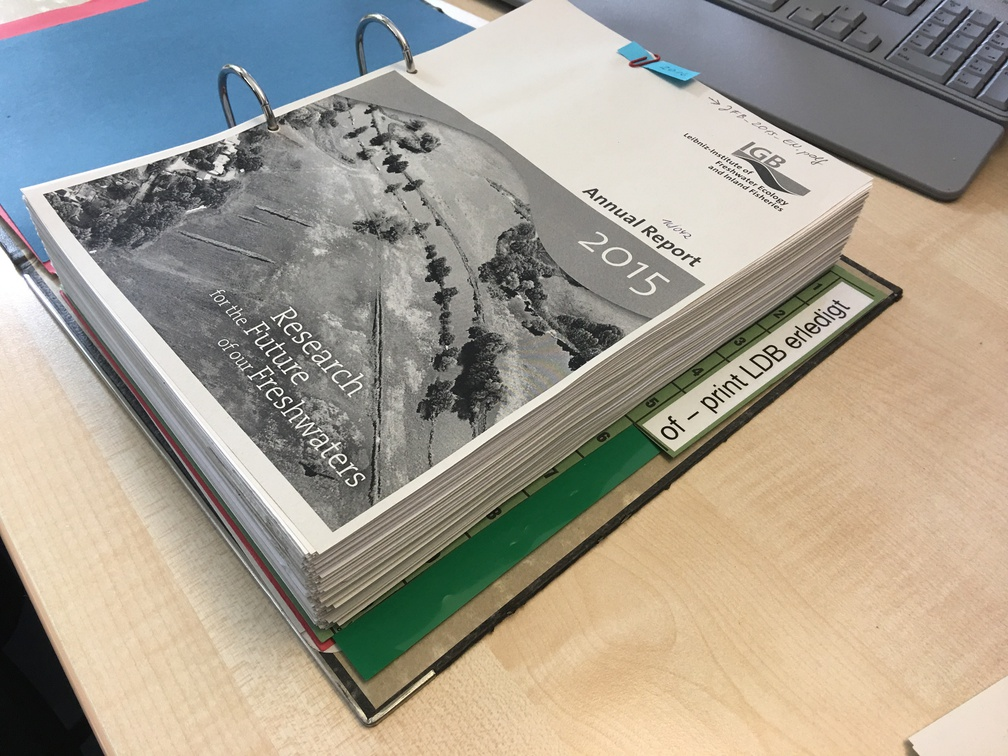
\includegraphics{igb/img/publikationen.jpg}
\end{center}

Auf dem Foto sieht man die ausgedruckten Titelseiten aller am Institut
erstellten Publikationen im Jahr 2016. Ich sehe sie auch als ein
Ergebnis der von Bibliotheken bereitgestellten gemeinsamen und lokalen
Infrastrukturen, ohne die Forschung nicht möglich wäre und die hier
wieder zurück in die Bibliothek finden.

\hypertarget{was-haben-sie-was-die-anderen-nicht-haben-warum-haben-sie-das-sollten-andere-es-auch-in-ihren-bibliotheken-haben}{%
\subsubsection*{Was haben Sie, was die anderen nicht haben? Warum haben Sie
das? Sollten andere es auch in ihren Bibliotheken
haben?}\label{was-haben-sie-was-die-anderen-nicht-haben-warum-haben-sie-das-sollten-andere-es-auch-in-ihren-bibliotheken-haben}}

\begin{center}
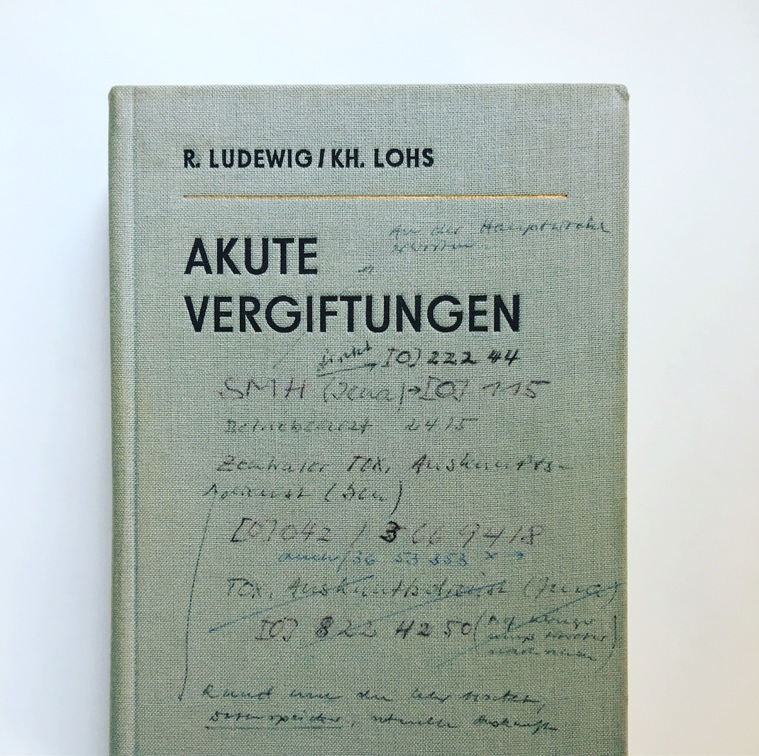
\includegraphics{igb/img/vergiftungen.jpg}
\end{center}

Auch wenn es das absolute No-Go ist, muss ich zugeben: Ich bin ein Fan
von Benutzungsspuren. Dieses Buch haben wir zufällig bei der
Bestandsdurchsicht gefunden. Elektronische Medien, für die wir heute den
Großteil unseres Budgets ausgeben, haben diese Spuren nicht. Bei allen
Vorteilen, die digitale Medien haben, vermisse ich es ein wenig, dass
Dateien niemals Geschichten erzählen werden können.

\hypertarget{ihre-bibliothek-name-adresse-spezialisierung-was-man-noch-uxfcber-sie-wissen-sollte}{%
\subsubsection*{Ihre Bibliothek (Name, Adresse, Spezialisierung, was man noch
über sie wissen
sollte)?}\label{ihre-bibliothek-name-adresse-spezialisierung-was-man-noch-uxfcber-sie-wissen-sollte}}

Bibliothek des Leibniz-Instituts für Gewässerökologie und
Binnenfischerei (IGB) im Forschungsverbund Berlin e.\,V., am Nordufer des
Müggelsees in Berlin-Friedrichshagen.

%autor
\begin{center}\rule{0.5\linewidth}{\linethickness}\end{center}

\textbf{Lydia Koglin}, nach geisteswissenschaftlichem Studium und
bibliothekswissenschaftlicher Ausbildung an einer Universitätsbibliothek
jetzt Leiterin einer Two-and-half-Woman-Bibliothek eines
umweltwissenschaftlichen Forschungsinstituts.
% !TEX root = ../master.tex

\vspace*{.5cm}
\section{Bibliothek des Leibniz-Instituts für Gewässerökologie und Binnenfischerei}
\begin{center}
\emph{Lydia Koglin}
\end{center}
\vspace*{1cm}

%body
\hypertarget{zeigen-sie-uns-den-ort-in-ihrer-bibliothek-an-dem-sie-die-meiste-zeit-verbringen.-was-ist-das-fuxfcr-ein-ort-wieso-sind-sie-die-meiste-zeit-dort}{%
\subsubsection*{Zeigen Sie uns den Ort in Ihrer Bibliothek, an dem Sie die
meiste Zeit verbringen. Was ist das für ein Ort? Wieso sind Sie die
meiste Zeit
dort?}\label{zeigen-sie-uns-den-ort-in-ihrer-bibliothek-an-dem-sie-die-meiste-zeit-verbringen.-was-ist-das-fuxfcr-ein-ort-wieso-sind-sie-die-meiste-zeit-dort}}

\begin{center}
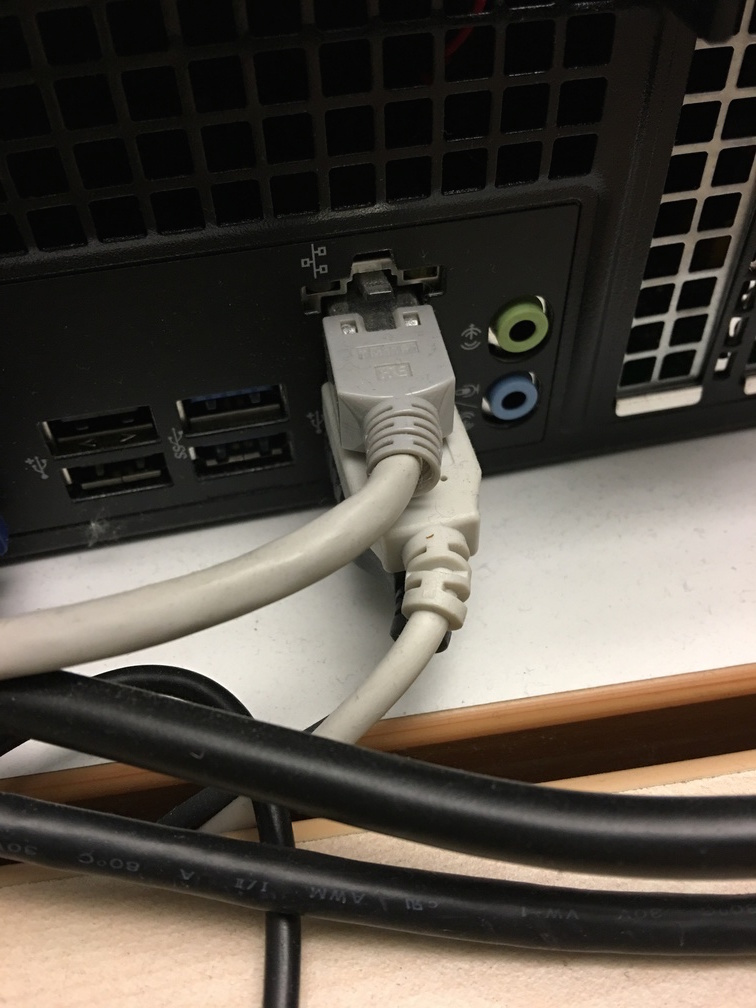
\includegraphics{igb/img/internet.jpg}
\end{center}

Zweifelsohne verbringen wir die meiste Zeit irgendwo im Netz. Wenn das
Netz ausfällt -- was es glücklicherweise selten macht --, merkt man das
erst richtig. Gut, dass es dann noch ein paar Bücherregale gibt, in
denen man mal wieder Ordnung schaffen kann.

\hypertarget{was-wuxfcrden-sie-vermissen-wenn-es-nicht-mehr-da-wuxe4re-wieso-wuxfcrden-sie-es-vermissen}{%
\subsubsection*{Was würden Sie vermissen, wenn es nicht mehr da wäre? Wieso
würden Sie es
vermissen?}\label{was-wuxfcrden-sie-vermissen-wenn-es-nicht-mehr-da-wuxe4re-wieso-wuxfcrden-sie-es-vermissen}}

\begin{center}
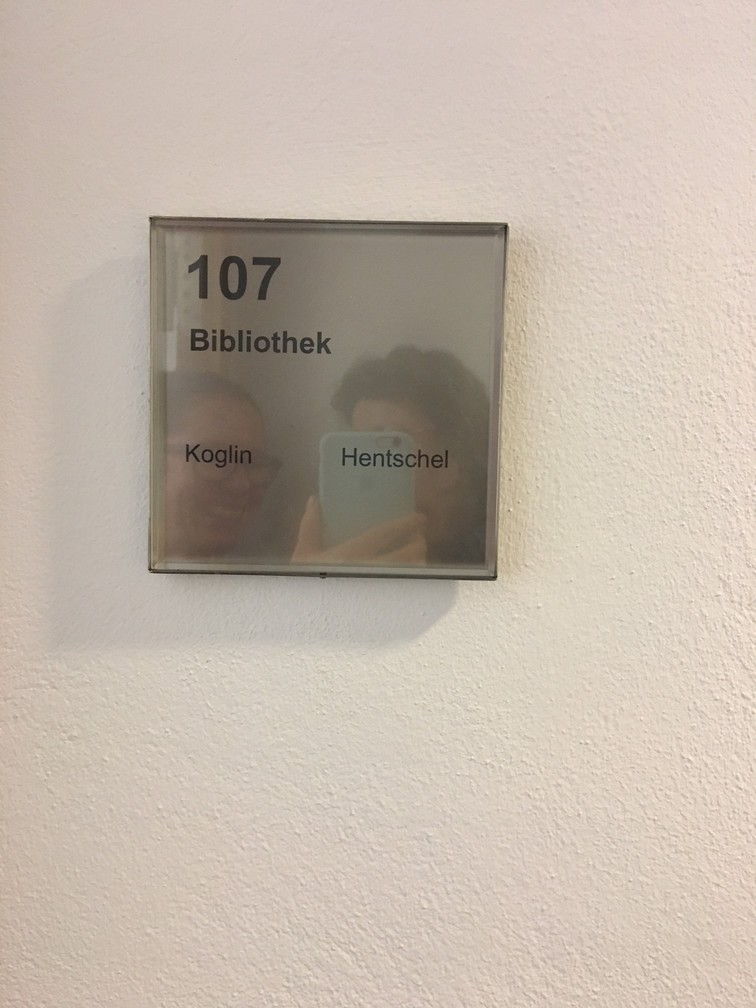
\includegraphics{igb/img/bibliothek.jpg}
\end{center}

Meine Kolleginnen. Wir sind eine Two-Persons-Library mit Hilfskraft und
ich habe einen sehr großen Respekt für Kolleginnen aus OPLs, die alles
alleine stemmen.

\hypertarget{was-stuxf6rt-sie-an-ihrer-bibliothek-beziehungsweise-was-wuxfcrden-sie-gerne-verbessern-wieso-stuxf6rt-sie-das-jetzt-noch}{%
\subsubsection*{Was stört Sie an Ihrer Bibliothek beziehungsweise was würden
Sie gerne verbessern? Wieso stört Sie das jetzt
(noch)?}\label{was-stuxf6rt-sie-an-ihrer-bibliothek-beziehungsweise-was-wuxfcrden-sie-gerne-verbessern-wieso-stuxf6rt-sie-das-jetzt-noch}}

\begin{center}
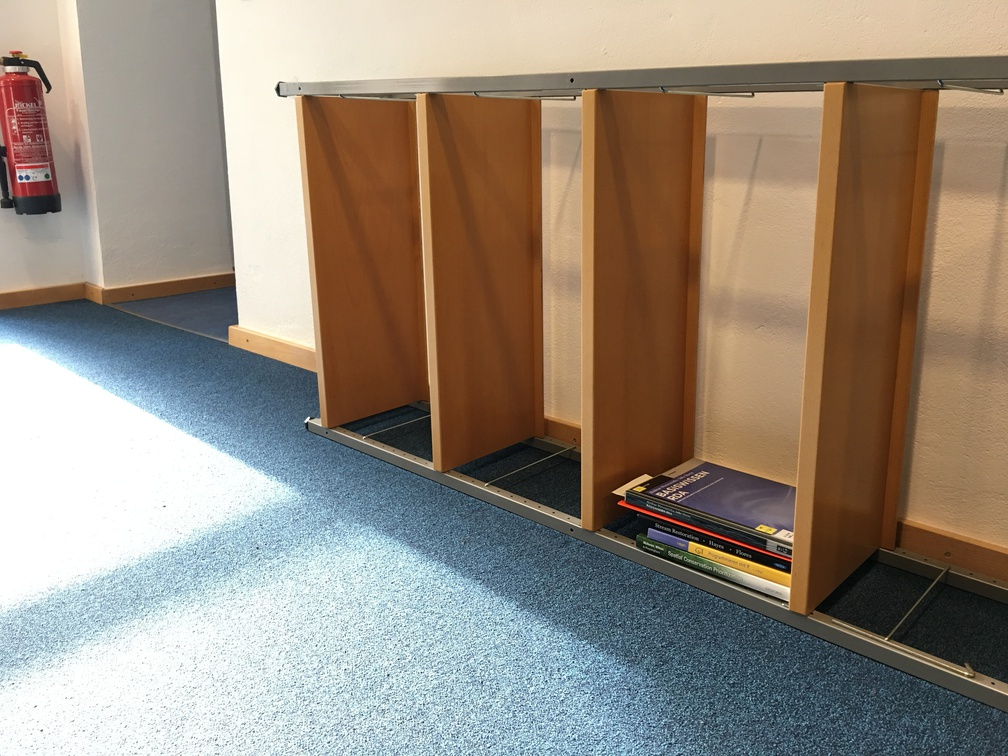
\includegraphics{igb/img/regal.jpg}
\end{center}

Wir sind gerade bei einem Projekt, bei dem wir mehrere tausend Bücher
umstellen. Physische Medien sind in ihrer Verwaltung, Bearbeitung und
täglichen Handhabung sehr aufwendig. Irgendwann dachte ich mal -- in den
Anfangsjahren der bibliothekarischen Tätigkeit -- so ein Regal ist
schnell umgeräumt oder ein paar Bücher schnell neu signiert. But, boy,
was I wrong\ldots{}

\hypertarget{zeigen-sie-uns-spuren-der-bibliotheksnutzung.-gibt-es-dazu-eine-geschichte}{%
\subsubsection*{Zeigen Sie uns Spuren der Bibliotheksnutzung. Gibt es dazu eine
Geschichte?}\label{zeigen-sie-uns-spuren-der-bibliotheksnutzung.-gibt-es-dazu-eine-geschichte}}

\begin{center}
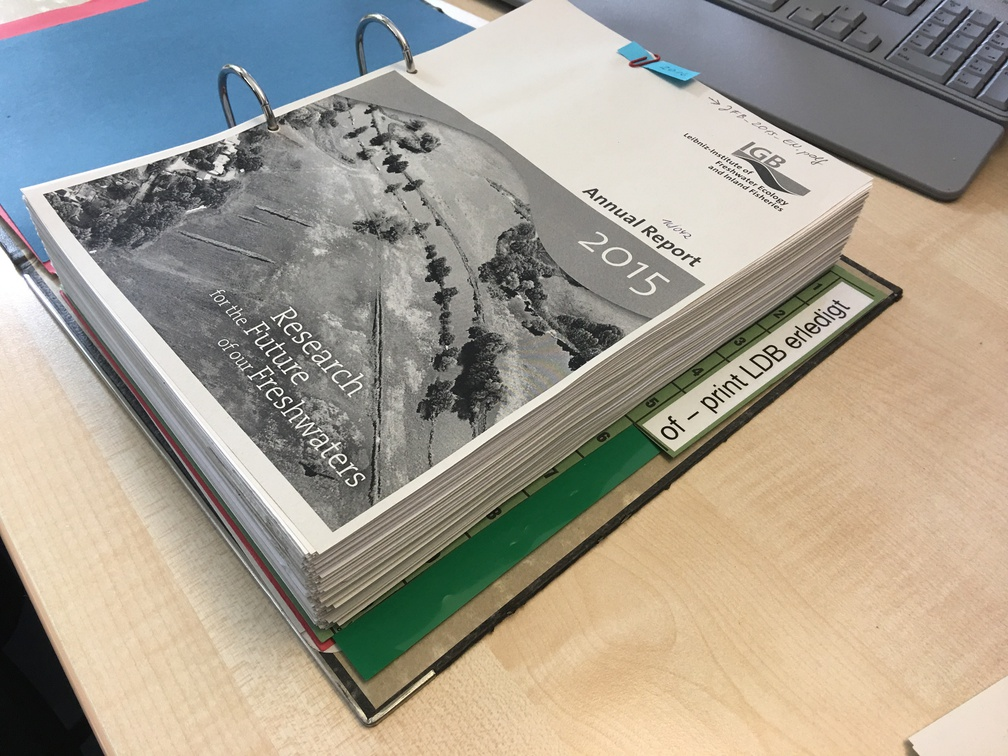
\includegraphics{igb/img/publikationen.jpg}
\end{center}

Auf dem Foto sieht man die ausgedruckten Titelseiten aller am Institut
erstellten Publikationen im Jahr 2016. Ich sehe sie auch als ein
Ergebnis der von Bibliotheken bereitgestellten gemeinsamen und lokalen
Infrastrukturen, ohne die Forschung nicht möglich wäre und die hier
wieder zurück in die Bibliothek finden.

\hypertarget{was-haben-sie-was-die-anderen-nicht-haben-warum-haben-sie-das-sollten-andere-es-auch-in-ihren-bibliotheken-haben}{%
\subsubsection*{Was haben Sie, was die anderen nicht haben? Warum haben Sie
das? Sollten andere es auch in ihren Bibliotheken
haben?}\label{was-haben-sie-was-die-anderen-nicht-haben-warum-haben-sie-das-sollten-andere-es-auch-in-ihren-bibliotheken-haben}}

\begin{center}
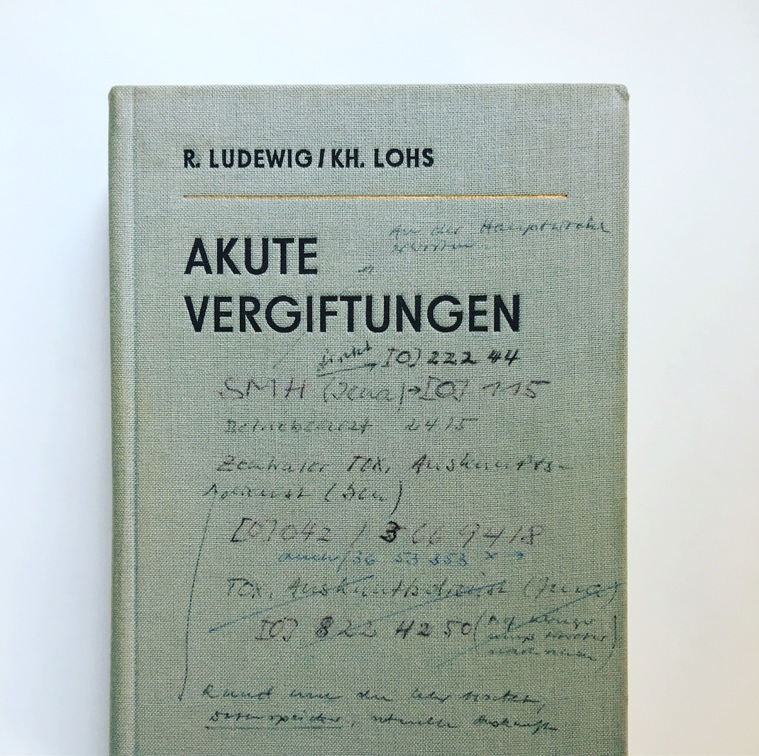
\includegraphics{igb/img/vergiftungen.jpg}
\end{center}

Auch wenn es das absolute No-Go ist, muss ich zugeben: Ich bin ein Fan
von Benutzungsspuren. Dieses Buch haben wir zufällig bei der
Bestandsdurchsicht gefunden. Elektronische Medien, für die wir heute den
Großteil unseres Budgets ausgeben, haben diese Spuren nicht. Bei allen
Vorteilen, die digitale Medien haben, vermisse ich es ein wenig, dass
Dateien niemals Geschichten erzählen werden können.

\hypertarget{ihre-bibliothek-name-adresse-spezialisierung-was-man-noch-uxfcber-sie-wissen-sollte}{%
\subsubsection*{Ihre Bibliothek (Name, Adresse, Spezialisierung, was man noch
über sie wissen
sollte)?}\label{ihre-bibliothek-name-adresse-spezialisierung-was-man-noch-uxfcber-sie-wissen-sollte}}

Bibliothek des Leibniz-Instituts für Gewässerökologie und
Binnenfischerei (IGB) im Forschungsverbund Berlin e.\,V., am Nordufer des
Müggelsees in Berlin-Friedrichshagen.

%autor
\begin{center}\rule{0.5\linewidth}{\linethickness}\end{center}

\textbf{Lydia Koglin}, nach geisteswissenschaftlichem Studium und
bibliothekswissenschaftlicher Ausbildung an einer Universitätsbibliothek
jetzt Leiterin einer Two-and-half-Woman-Bibliothek eines
umweltwissenschaftlichen Forschungsinstituts.
% !TEX root = ../master.tex

\vspace*{.5cm}
\section{Bibliothek des Leibniz-Instituts für Gewässerökologie und Binnenfischerei}
\begin{center}
\emph{Lydia Koglin}
\end{center}
\vspace*{1cm}

%body
\hypertarget{zeigen-sie-uns-den-ort-in-ihrer-bibliothek-an-dem-sie-die-meiste-zeit-verbringen.-was-ist-das-fuxfcr-ein-ort-wieso-sind-sie-die-meiste-zeit-dort}{%
\subsubsection*{Zeigen Sie uns den Ort in Ihrer Bibliothek, an dem Sie die
meiste Zeit verbringen. Was ist das für ein Ort? Wieso sind Sie die
meiste Zeit
dort?}\label{zeigen-sie-uns-den-ort-in-ihrer-bibliothek-an-dem-sie-die-meiste-zeit-verbringen.-was-ist-das-fuxfcr-ein-ort-wieso-sind-sie-die-meiste-zeit-dort}}

\begin{center}
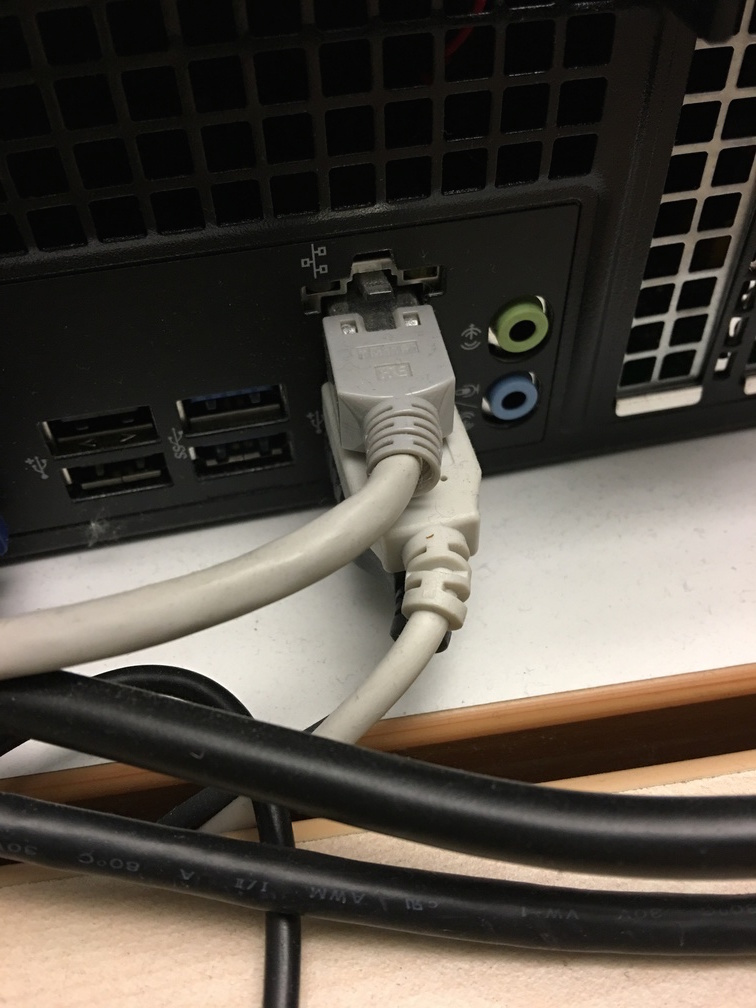
\includegraphics{igb/img/internet.jpg}
\end{center}

Zweifelsohne verbringen wir die meiste Zeit irgendwo im Netz. Wenn das
Netz ausfällt -- was es glücklicherweise selten macht --, merkt man das
erst richtig. Gut, dass es dann noch ein paar Bücherregale gibt, in
denen man mal wieder Ordnung schaffen kann.

\hypertarget{was-wuxfcrden-sie-vermissen-wenn-es-nicht-mehr-da-wuxe4re-wieso-wuxfcrden-sie-es-vermissen}{%
\subsubsection*{Was würden Sie vermissen, wenn es nicht mehr da wäre? Wieso
würden Sie es
vermissen?}\label{was-wuxfcrden-sie-vermissen-wenn-es-nicht-mehr-da-wuxe4re-wieso-wuxfcrden-sie-es-vermissen}}

\begin{center}
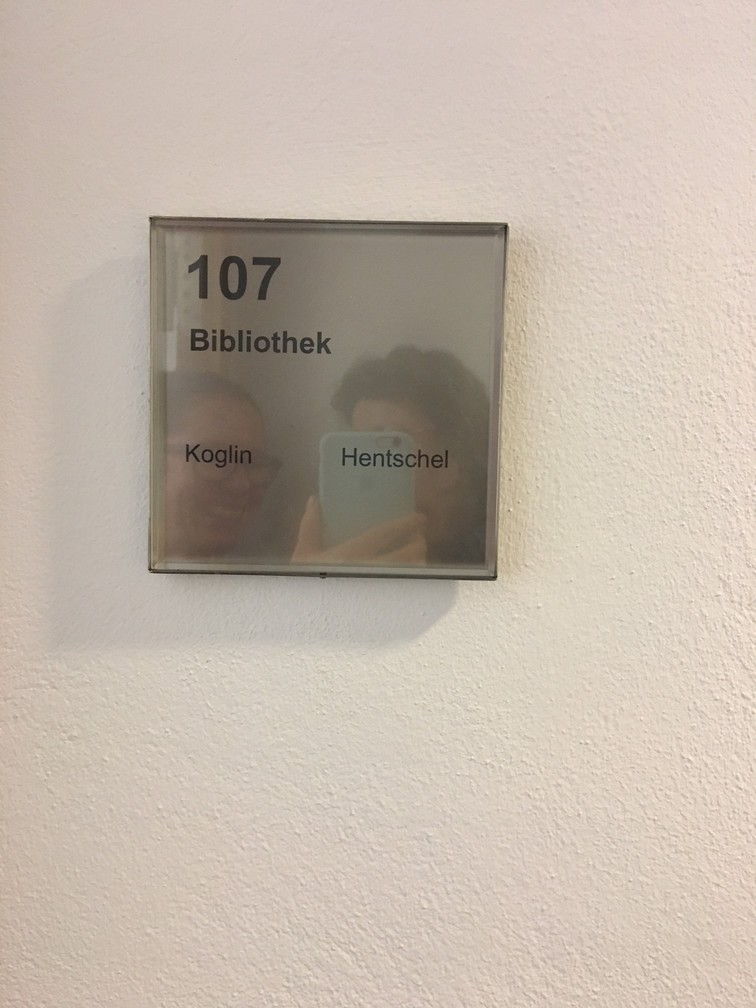
\includegraphics{igb/img/bibliothek.jpg}
\end{center}

Meine Kolleginnen. Wir sind eine Two-Persons-Library mit Hilfskraft und
ich habe einen sehr großen Respekt für Kolleginnen aus OPLs, die alles
alleine stemmen.

\hypertarget{was-stuxf6rt-sie-an-ihrer-bibliothek-beziehungsweise-was-wuxfcrden-sie-gerne-verbessern-wieso-stuxf6rt-sie-das-jetzt-noch}{%
\subsubsection*{Was stört Sie an Ihrer Bibliothek beziehungsweise was würden
Sie gerne verbessern? Wieso stört Sie das jetzt
(noch)?}\label{was-stuxf6rt-sie-an-ihrer-bibliothek-beziehungsweise-was-wuxfcrden-sie-gerne-verbessern-wieso-stuxf6rt-sie-das-jetzt-noch}}

\begin{center}
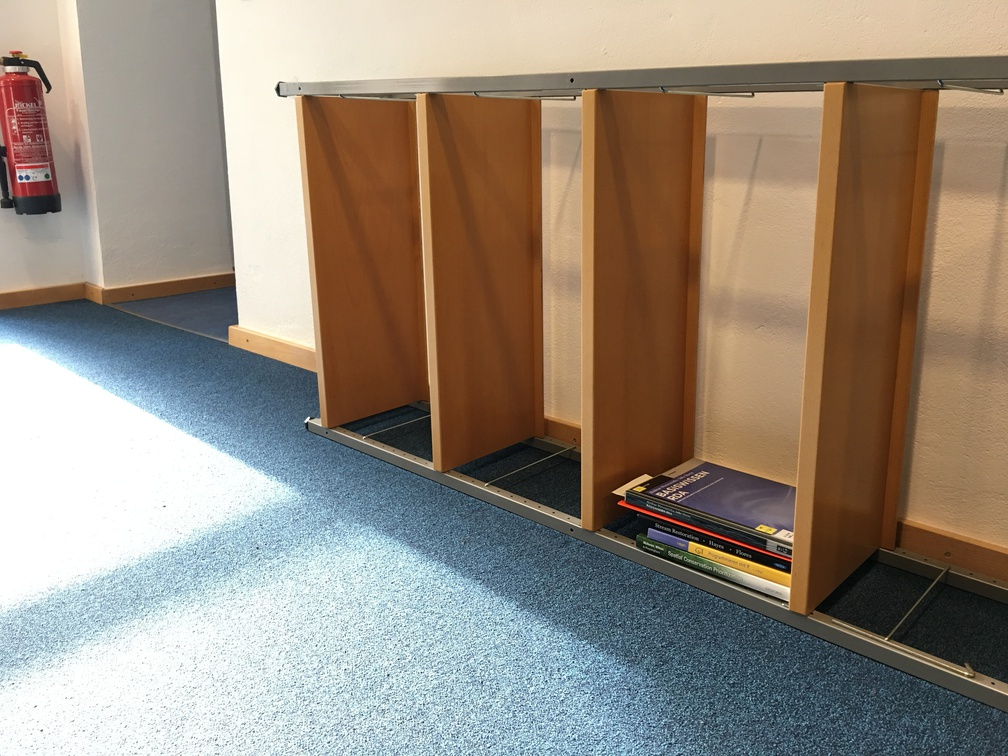
\includegraphics{igb/img/regal.jpg}
\end{center}

Wir sind gerade bei einem Projekt, bei dem wir mehrere tausend Bücher
umstellen. Physische Medien sind in ihrer Verwaltung, Bearbeitung und
täglichen Handhabung sehr aufwendig. Irgendwann dachte ich mal -- in den
Anfangsjahren der bibliothekarischen Tätigkeit -- so ein Regal ist
schnell umgeräumt oder ein paar Bücher schnell neu signiert. But, boy,
was I wrong\ldots{}

\hypertarget{zeigen-sie-uns-spuren-der-bibliotheksnutzung.-gibt-es-dazu-eine-geschichte}{%
\subsubsection*{Zeigen Sie uns Spuren der Bibliotheksnutzung. Gibt es dazu eine
Geschichte?}\label{zeigen-sie-uns-spuren-der-bibliotheksnutzung.-gibt-es-dazu-eine-geschichte}}

\begin{center}
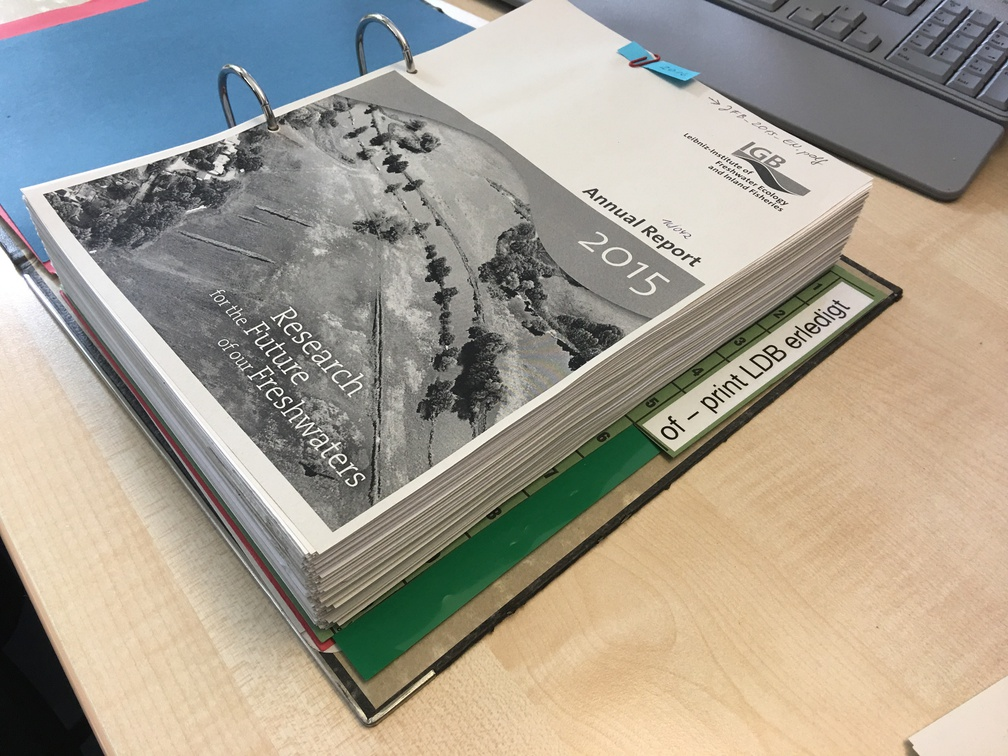
\includegraphics{igb/img/publikationen.jpg}
\end{center}

Auf dem Foto sieht man die ausgedruckten Titelseiten aller am Institut
erstellten Publikationen im Jahr 2016. Ich sehe sie auch als ein
Ergebnis der von Bibliotheken bereitgestellten gemeinsamen und lokalen
Infrastrukturen, ohne die Forschung nicht möglich wäre und die hier
wieder zurück in die Bibliothek finden.

\hypertarget{was-haben-sie-was-die-anderen-nicht-haben-warum-haben-sie-das-sollten-andere-es-auch-in-ihren-bibliotheken-haben}{%
\subsubsection*{Was haben Sie, was die anderen nicht haben? Warum haben Sie
das? Sollten andere es auch in ihren Bibliotheken
haben?}\label{was-haben-sie-was-die-anderen-nicht-haben-warum-haben-sie-das-sollten-andere-es-auch-in-ihren-bibliotheken-haben}}

\begin{center}
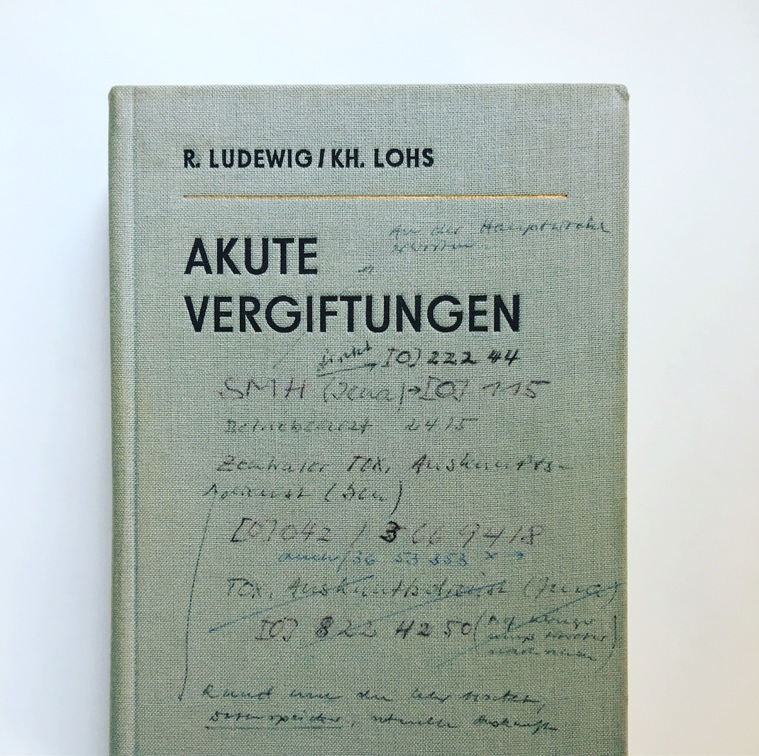
\includegraphics{igb/img/vergiftungen.jpg}
\end{center}

Auch wenn es das absolute No-Go ist, muss ich zugeben: Ich bin ein Fan
von Benutzungsspuren. Dieses Buch haben wir zufällig bei der
Bestandsdurchsicht gefunden. Elektronische Medien, für die wir heute den
Großteil unseres Budgets ausgeben, haben diese Spuren nicht. Bei allen
Vorteilen, die digitale Medien haben, vermisse ich es ein wenig, dass
Dateien niemals Geschichten erzählen werden können.

\hypertarget{ihre-bibliothek-name-adresse-spezialisierung-was-man-noch-uxfcber-sie-wissen-sollte}{%
\subsubsection*{Ihre Bibliothek (Name, Adresse, Spezialisierung, was man noch
über sie wissen
sollte)?}\label{ihre-bibliothek-name-adresse-spezialisierung-was-man-noch-uxfcber-sie-wissen-sollte}}

Bibliothek des Leibniz-Instituts für Gewässerökologie und
Binnenfischerei (IGB) im Forschungsverbund Berlin e.\,V., am Nordufer des
Müggelsees in Berlin-Friedrichshagen.

%autor
\begin{center}\rule{0.5\linewidth}{\linethickness}\end{center}

\textbf{Lydia Koglin}, nach geisteswissenschaftlichem Studium und
bibliothekswissenschaftlicher Ausbildung an einer Universitätsbibliothek
jetzt Leiterin einer Two-and-half-Woman-Bibliothek eines
umweltwissenschaftlichen Forschungsinstituts.
% !TEX root = ../master.tex

\vspace*{.5cm}
\section{Bibliothek des Leibniz-Instituts für Gewässerökologie und Binnenfischerei}
\begin{center}
\emph{Lydia Koglin}
\end{center}
\vspace*{1cm}

%body
\hypertarget{zeigen-sie-uns-den-ort-in-ihrer-bibliothek-an-dem-sie-die-meiste-zeit-verbringen.-was-ist-das-fuxfcr-ein-ort-wieso-sind-sie-die-meiste-zeit-dort}{%
\subsubsection*{Zeigen Sie uns den Ort in Ihrer Bibliothek, an dem Sie die
meiste Zeit verbringen. Was ist das für ein Ort? Wieso sind Sie die
meiste Zeit
dort?}\label{zeigen-sie-uns-den-ort-in-ihrer-bibliothek-an-dem-sie-die-meiste-zeit-verbringen.-was-ist-das-fuxfcr-ein-ort-wieso-sind-sie-die-meiste-zeit-dort}}

\begin{center}
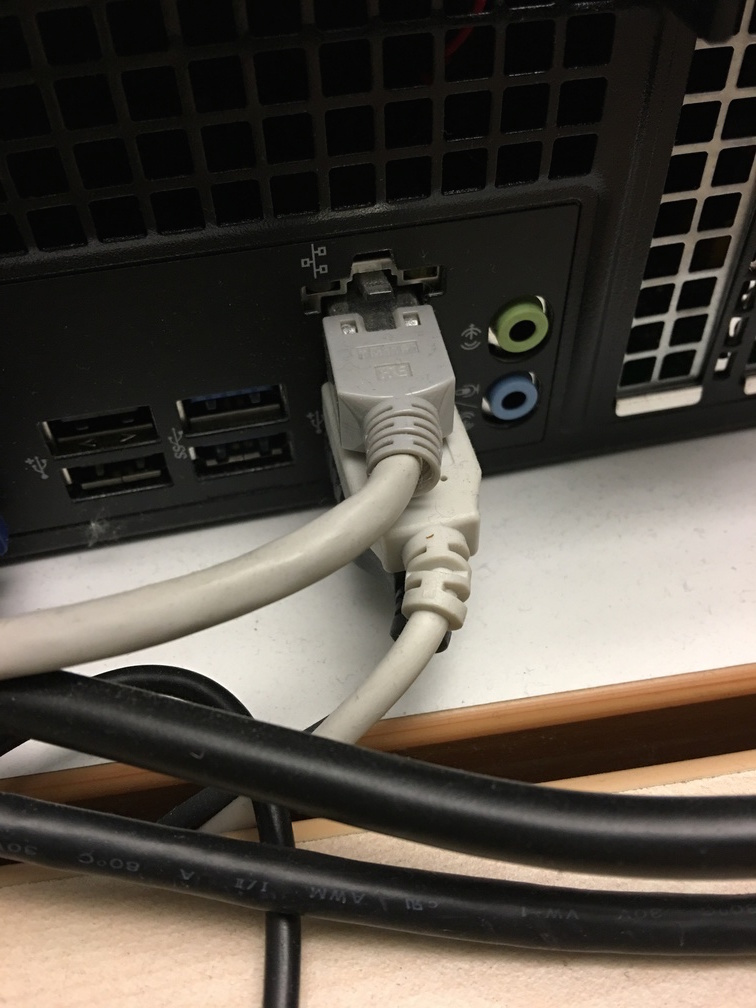
\includegraphics{igb/img/internet.jpg}
\end{center}

Zweifelsohne verbringen wir die meiste Zeit irgendwo im Netz. Wenn das
Netz ausfällt -- was es glücklicherweise selten macht --, merkt man das
erst richtig. Gut, dass es dann noch ein paar Bücherregale gibt, in
denen man mal wieder Ordnung schaffen kann.

\hypertarget{was-wuxfcrden-sie-vermissen-wenn-es-nicht-mehr-da-wuxe4re-wieso-wuxfcrden-sie-es-vermissen}{%
\subsubsection*{Was würden Sie vermissen, wenn es nicht mehr da wäre? Wieso
würden Sie es
vermissen?}\label{was-wuxfcrden-sie-vermissen-wenn-es-nicht-mehr-da-wuxe4re-wieso-wuxfcrden-sie-es-vermissen}}

\begin{center}
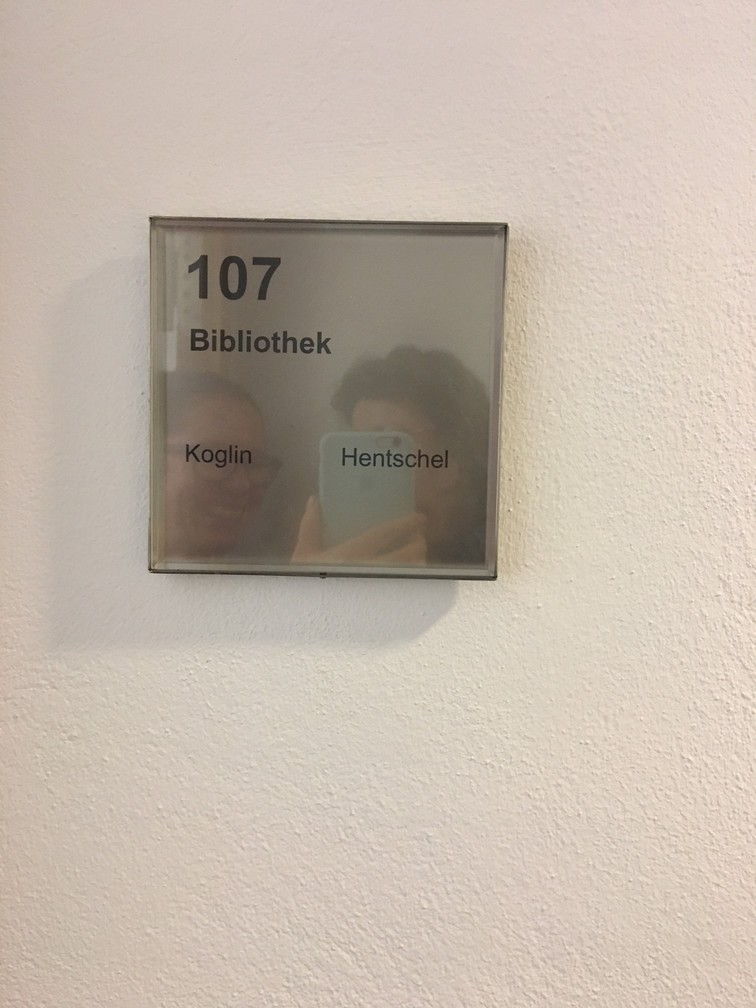
\includegraphics{igb/img/bibliothek.jpg}
\end{center}

Meine Kolleginnen. Wir sind eine Two-Persons-Library mit Hilfskraft und
ich habe einen sehr großen Respekt für Kolleginnen aus OPLs, die alles
alleine stemmen.

\hypertarget{was-stuxf6rt-sie-an-ihrer-bibliothek-beziehungsweise-was-wuxfcrden-sie-gerne-verbessern-wieso-stuxf6rt-sie-das-jetzt-noch}{%
\subsubsection*{Was stört Sie an Ihrer Bibliothek beziehungsweise was würden
Sie gerne verbessern? Wieso stört Sie das jetzt
(noch)?}\label{was-stuxf6rt-sie-an-ihrer-bibliothek-beziehungsweise-was-wuxfcrden-sie-gerne-verbessern-wieso-stuxf6rt-sie-das-jetzt-noch}}

\begin{center}
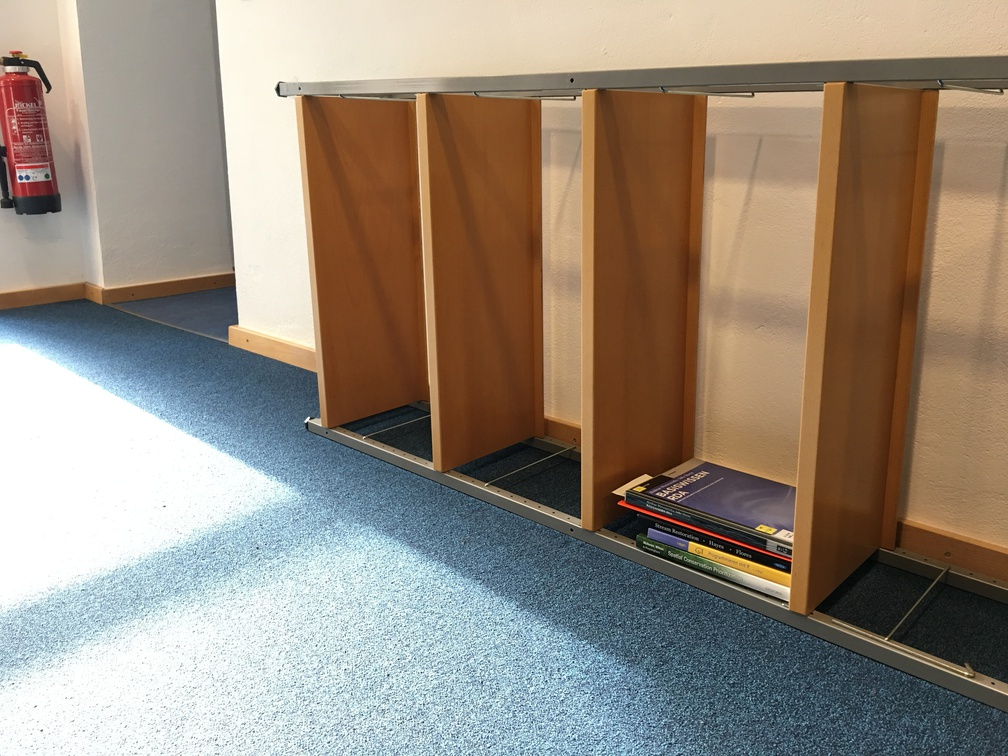
\includegraphics{igb/img/regal.jpg}
\end{center}

Wir sind gerade bei einem Projekt, bei dem wir mehrere tausend Bücher
umstellen. Physische Medien sind in ihrer Verwaltung, Bearbeitung und
täglichen Handhabung sehr aufwendig. Irgendwann dachte ich mal -- in den
Anfangsjahren der bibliothekarischen Tätigkeit -- so ein Regal ist
schnell umgeräumt oder ein paar Bücher schnell neu signiert. But, boy,
was I wrong\ldots{}

\hypertarget{zeigen-sie-uns-spuren-der-bibliotheksnutzung.-gibt-es-dazu-eine-geschichte}{%
\subsubsection*{Zeigen Sie uns Spuren der Bibliotheksnutzung. Gibt es dazu eine
Geschichte?}\label{zeigen-sie-uns-spuren-der-bibliotheksnutzung.-gibt-es-dazu-eine-geschichte}}

\begin{center}
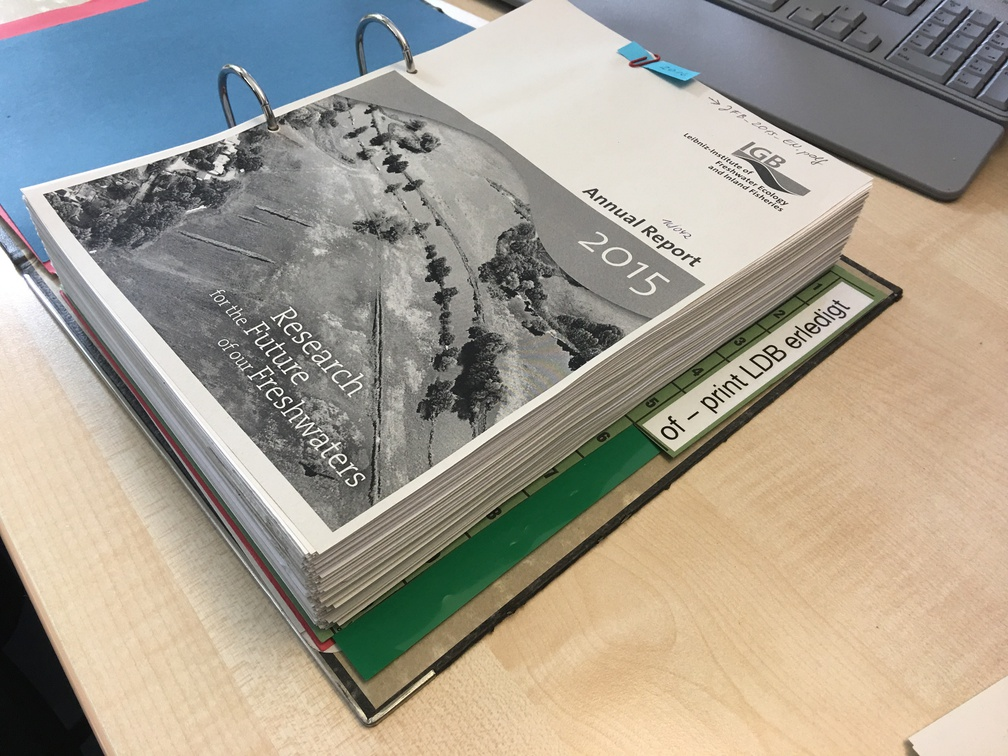
\includegraphics{igb/img/publikationen.jpg}
\end{center}

Auf dem Foto sieht man die ausgedruckten Titelseiten aller am Institut
erstellten Publikationen im Jahr 2016. Ich sehe sie auch als ein
Ergebnis der von Bibliotheken bereitgestellten gemeinsamen und lokalen
Infrastrukturen, ohne die Forschung nicht möglich wäre und die hier
wieder zurück in die Bibliothek finden.

\hypertarget{was-haben-sie-was-die-anderen-nicht-haben-warum-haben-sie-das-sollten-andere-es-auch-in-ihren-bibliotheken-haben}{%
\subsubsection*{Was haben Sie, was die anderen nicht haben? Warum haben Sie
das? Sollten andere es auch in ihren Bibliotheken
haben?}\label{was-haben-sie-was-die-anderen-nicht-haben-warum-haben-sie-das-sollten-andere-es-auch-in-ihren-bibliotheken-haben}}

\begin{center}
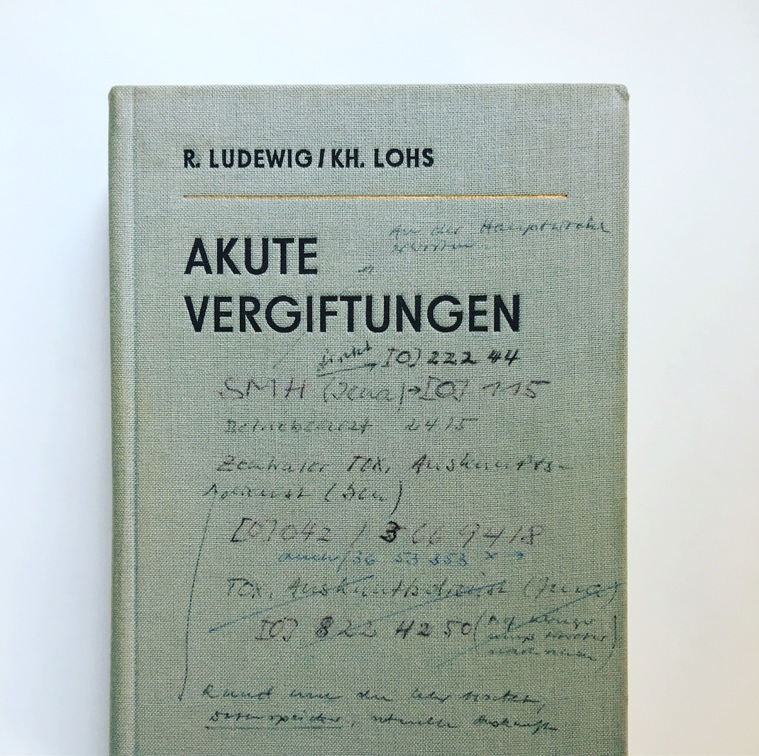
\includegraphics{igb/img/vergiftungen.jpg}
\end{center}

Auch wenn es das absolute No-Go ist, muss ich zugeben: Ich bin ein Fan
von Benutzungsspuren. Dieses Buch haben wir zufällig bei der
Bestandsdurchsicht gefunden. Elektronische Medien, für die wir heute den
Großteil unseres Budgets ausgeben, haben diese Spuren nicht. Bei allen
Vorteilen, die digitale Medien haben, vermisse ich es ein wenig, dass
Dateien niemals Geschichten erzählen werden können.

\hypertarget{ihre-bibliothek-name-adresse-spezialisierung-was-man-noch-uxfcber-sie-wissen-sollte}{%
\subsubsection*{Ihre Bibliothek (Name, Adresse, Spezialisierung, was man noch
über sie wissen
sollte)?}\label{ihre-bibliothek-name-adresse-spezialisierung-was-man-noch-uxfcber-sie-wissen-sollte}}

Bibliothek des Leibniz-Instituts für Gewässerökologie und
Binnenfischerei (IGB) im Forschungsverbund Berlin e.\,V., am Nordufer des
Müggelsees in Berlin-Friedrichshagen.

%autor
\begin{center}\rule{0.5\linewidth}{\linethickness}\end{center}

\textbf{Lydia Koglin}, nach geisteswissenschaftlichem Studium und
bibliothekswissenschaftlicher Ausbildung an einer Universitätsbibliothek
jetzt Leiterin einer Two-and-half-Woman-Bibliothek eines
umweltwissenschaftlichen Forschungsinstituts.
% !TEX root = ../master.tex

\vspace*{.5cm}
\section{Bibliothek des Leibniz-Instituts für Gewässerökologie und Binnenfischerei}
\begin{center}
\emph{Lydia Koglin}
\end{center}
\vspace*{1cm}

%body
\hypertarget{zeigen-sie-uns-den-ort-in-ihrer-bibliothek-an-dem-sie-die-meiste-zeit-verbringen.-was-ist-das-fuxfcr-ein-ort-wieso-sind-sie-die-meiste-zeit-dort}{%
\subsubsection*{Zeigen Sie uns den Ort in Ihrer Bibliothek, an dem Sie die
meiste Zeit verbringen. Was ist das für ein Ort? Wieso sind Sie die
meiste Zeit
dort?}\label{zeigen-sie-uns-den-ort-in-ihrer-bibliothek-an-dem-sie-die-meiste-zeit-verbringen.-was-ist-das-fuxfcr-ein-ort-wieso-sind-sie-die-meiste-zeit-dort}}

\begin{center}
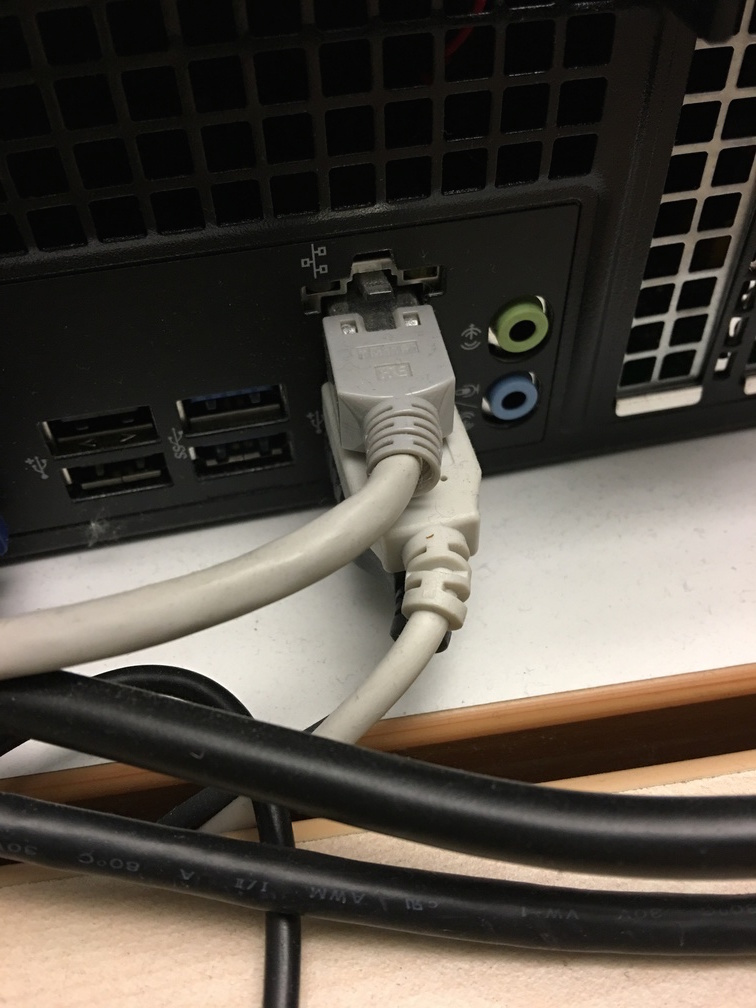
\includegraphics{igb/img/internet.jpg}
\end{center}

Zweifelsohne verbringen wir die meiste Zeit irgendwo im Netz. Wenn das
Netz ausfällt -- was es glücklicherweise selten macht --, merkt man das
erst richtig. Gut, dass es dann noch ein paar Bücherregale gibt, in
denen man mal wieder Ordnung schaffen kann.

\hypertarget{was-wuxfcrden-sie-vermissen-wenn-es-nicht-mehr-da-wuxe4re-wieso-wuxfcrden-sie-es-vermissen}{%
\subsubsection*{Was würden Sie vermissen, wenn es nicht mehr da wäre? Wieso
würden Sie es
vermissen?}\label{was-wuxfcrden-sie-vermissen-wenn-es-nicht-mehr-da-wuxe4re-wieso-wuxfcrden-sie-es-vermissen}}

\begin{center}
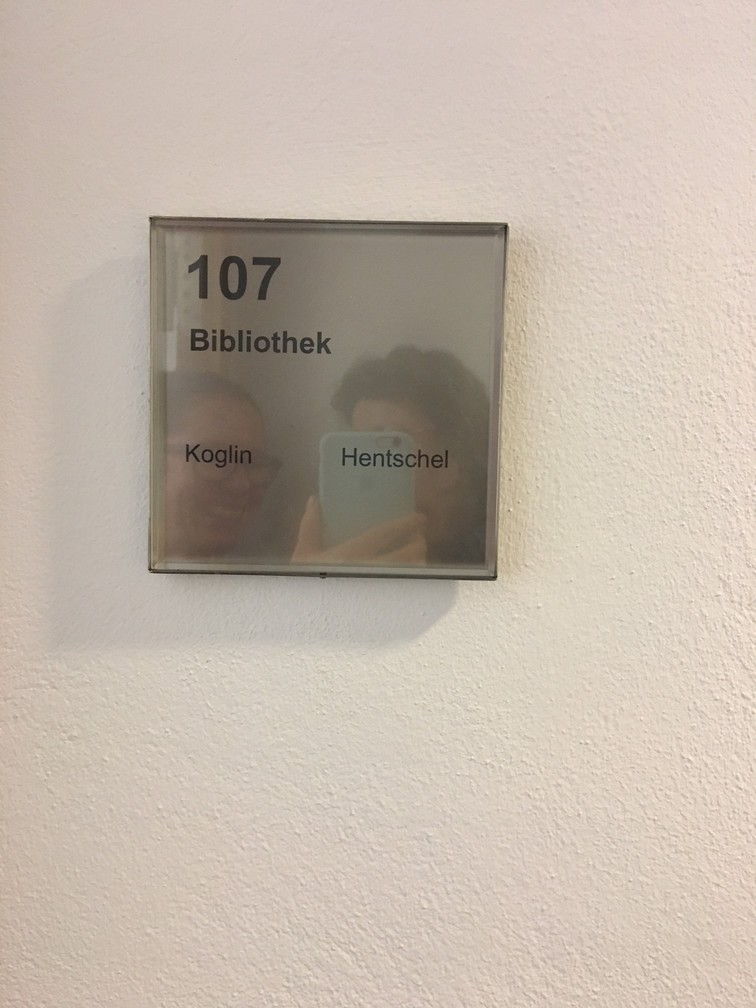
\includegraphics{igb/img/bibliothek.jpg}
\end{center}

Meine Kolleginnen. Wir sind eine Two-Persons-Library mit Hilfskraft und
ich habe einen sehr großen Respekt für Kolleginnen aus OPLs, die alles
alleine stemmen.

\hypertarget{was-stuxf6rt-sie-an-ihrer-bibliothek-beziehungsweise-was-wuxfcrden-sie-gerne-verbessern-wieso-stuxf6rt-sie-das-jetzt-noch}{%
\subsubsection*{Was stört Sie an Ihrer Bibliothek beziehungsweise was würden
Sie gerne verbessern? Wieso stört Sie das jetzt
(noch)?}\label{was-stuxf6rt-sie-an-ihrer-bibliothek-beziehungsweise-was-wuxfcrden-sie-gerne-verbessern-wieso-stuxf6rt-sie-das-jetzt-noch}}

\begin{center}
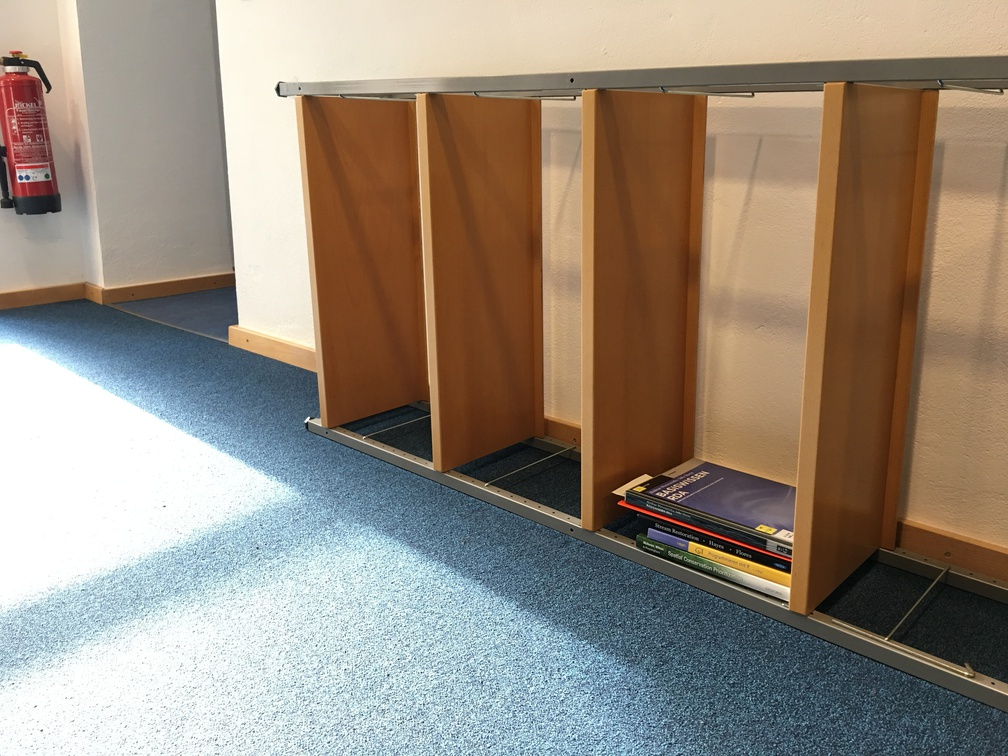
\includegraphics{igb/img/regal.jpg}
\end{center}

Wir sind gerade bei einem Projekt, bei dem wir mehrere tausend Bücher
umstellen. Physische Medien sind in ihrer Verwaltung, Bearbeitung und
täglichen Handhabung sehr aufwendig. Irgendwann dachte ich mal -- in den
Anfangsjahren der bibliothekarischen Tätigkeit -- so ein Regal ist
schnell umgeräumt oder ein paar Bücher schnell neu signiert. But, boy,
was I wrong\ldots{}

\hypertarget{zeigen-sie-uns-spuren-der-bibliotheksnutzung.-gibt-es-dazu-eine-geschichte}{%
\subsubsection*{Zeigen Sie uns Spuren der Bibliotheksnutzung. Gibt es dazu eine
Geschichte?}\label{zeigen-sie-uns-spuren-der-bibliotheksnutzung.-gibt-es-dazu-eine-geschichte}}

\begin{center}
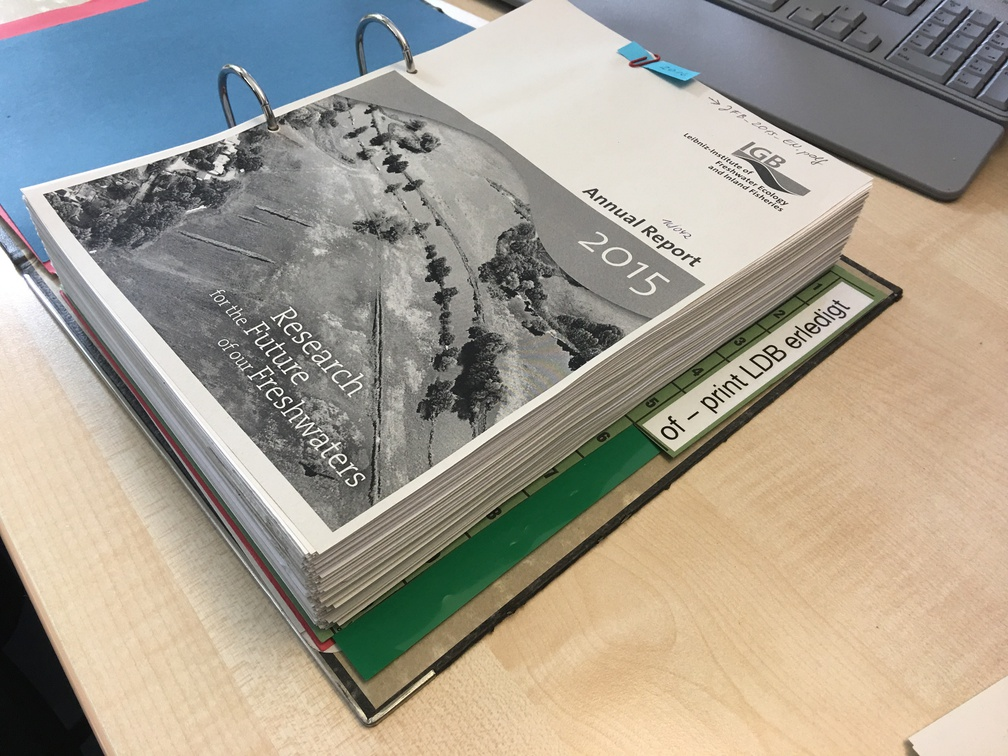
\includegraphics{igb/img/publikationen.jpg}
\end{center}

Auf dem Foto sieht man die ausgedruckten Titelseiten aller am Institut
erstellten Publikationen im Jahr 2016. Ich sehe sie auch als ein
Ergebnis der von Bibliotheken bereitgestellten gemeinsamen und lokalen
Infrastrukturen, ohne die Forschung nicht möglich wäre und die hier
wieder zurück in die Bibliothek finden.

\hypertarget{was-haben-sie-was-die-anderen-nicht-haben-warum-haben-sie-das-sollten-andere-es-auch-in-ihren-bibliotheken-haben}{%
\subsubsection*{Was haben Sie, was die anderen nicht haben? Warum haben Sie
das? Sollten andere es auch in ihren Bibliotheken
haben?}\label{was-haben-sie-was-die-anderen-nicht-haben-warum-haben-sie-das-sollten-andere-es-auch-in-ihren-bibliotheken-haben}}

\begin{center}
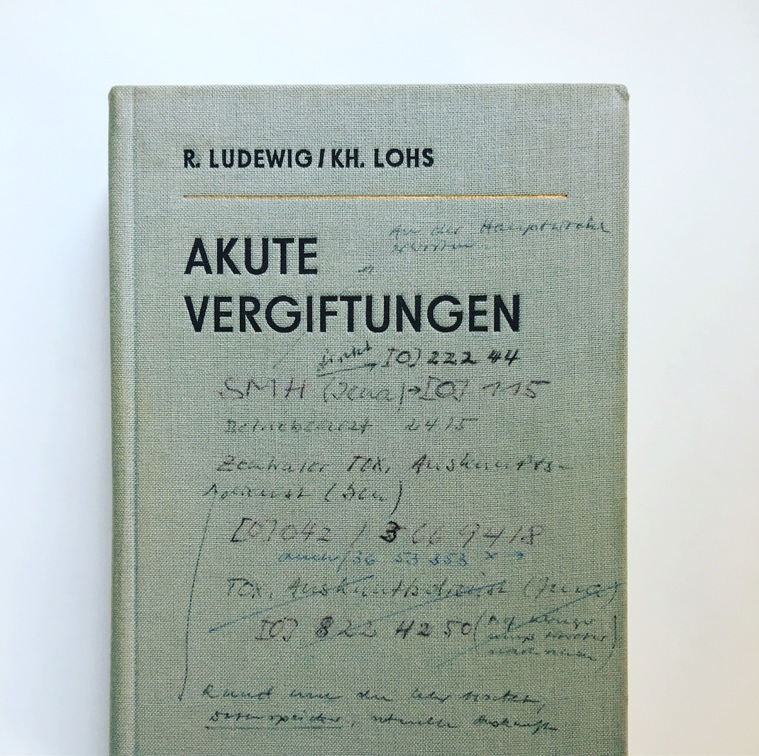
\includegraphics{igb/img/vergiftungen.jpg}
\end{center}

Auch wenn es das absolute No-Go ist, muss ich zugeben: Ich bin ein Fan
von Benutzungsspuren. Dieses Buch haben wir zufällig bei der
Bestandsdurchsicht gefunden. Elektronische Medien, für die wir heute den
Großteil unseres Budgets ausgeben, haben diese Spuren nicht. Bei allen
Vorteilen, die digitale Medien haben, vermisse ich es ein wenig, dass
Dateien niemals Geschichten erzählen werden können.

\hypertarget{ihre-bibliothek-name-adresse-spezialisierung-was-man-noch-uxfcber-sie-wissen-sollte}{%
\subsubsection*{Ihre Bibliothek (Name, Adresse, Spezialisierung, was man noch
über sie wissen
sollte)?}\label{ihre-bibliothek-name-adresse-spezialisierung-was-man-noch-uxfcber-sie-wissen-sollte}}

Bibliothek des Leibniz-Instituts für Gewässerökologie und
Binnenfischerei (IGB) im Forschungsverbund Berlin e.\,V., am Nordufer des
Müggelsees in Berlin-Friedrichshagen.

%autor
\begin{center}\rule{0.5\linewidth}{\linethickness}\end{center}

\textbf{Lydia Koglin}, nach geisteswissenschaftlichem Studium und
bibliothekswissenschaftlicher Ausbildung an einer Universitätsbibliothek
jetzt Leiterin einer Two-and-half-Woman-Bibliothek eines
umweltwissenschaftlichen Forschungsinstituts.
% !TEX root = ../master.tex

\vspace*{.5cm}
\section{Bibliothek des Leibniz-Instituts für Gewässerökologie und Binnenfischerei}
\begin{center}
\emph{Lydia Koglin}
\end{center}
\vspace*{1cm}

%body
\hypertarget{zeigen-sie-uns-den-ort-in-ihrer-bibliothek-an-dem-sie-die-meiste-zeit-verbringen.-was-ist-das-fuxfcr-ein-ort-wieso-sind-sie-die-meiste-zeit-dort}{%
\subsubsection*{Zeigen Sie uns den Ort in Ihrer Bibliothek, an dem Sie die
meiste Zeit verbringen. Was ist das für ein Ort? Wieso sind Sie die
meiste Zeit
dort?}\label{zeigen-sie-uns-den-ort-in-ihrer-bibliothek-an-dem-sie-die-meiste-zeit-verbringen.-was-ist-das-fuxfcr-ein-ort-wieso-sind-sie-die-meiste-zeit-dort}}

\begin{center}
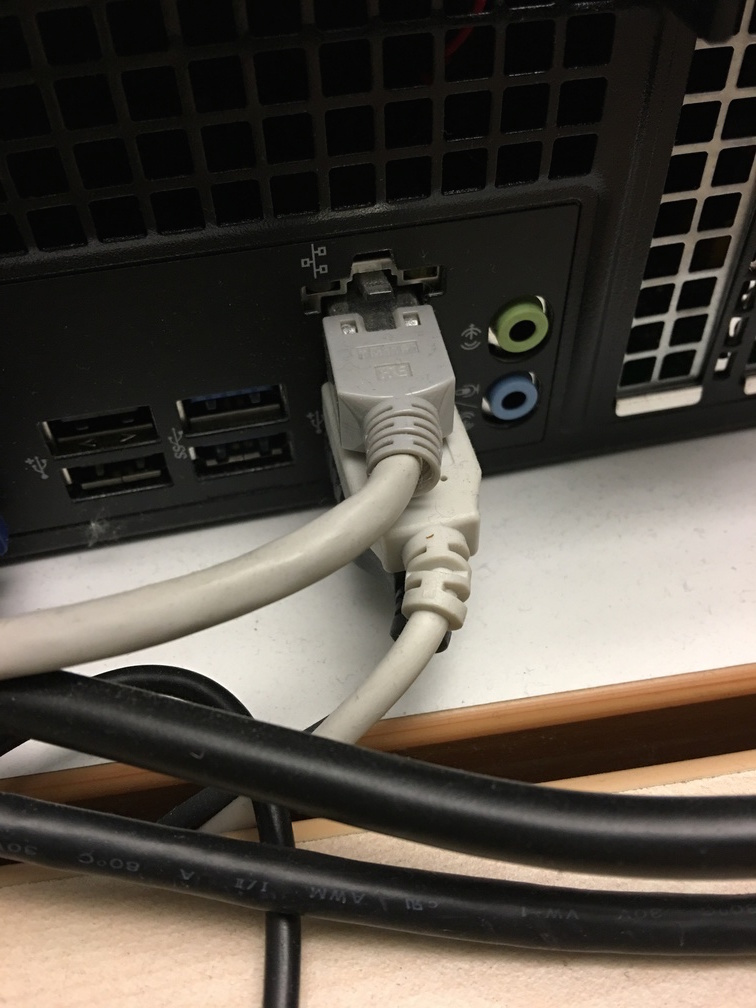
\includegraphics{igb/img/internet.jpg}
\end{center}

Zweifelsohne verbringen wir die meiste Zeit irgendwo im Netz. Wenn das
Netz ausfällt -- was es glücklicherweise selten macht --, merkt man das
erst richtig. Gut, dass es dann noch ein paar Bücherregale gibt, in
denen man mal wieder Ordnung schaffen kann.

\hypertarget{was-wuxfcrden-sie-vermissen-wenn-es-nicht-mehr-da-wuxe4re-wieso-wuxfcrden-sie-es-vermissen}{%
\subsubsection*{Was würden Sie vermissen, wenn es nicht mehr da wäre? Wieso
würden Sie es
vermissen?}\label{was-wuxfcrden-sie-vermissen-wenn-es-nicht-mehr-da-wuxe4re-wieso-wuxfcrden-sie-es-vermissen}}

\begin{center}
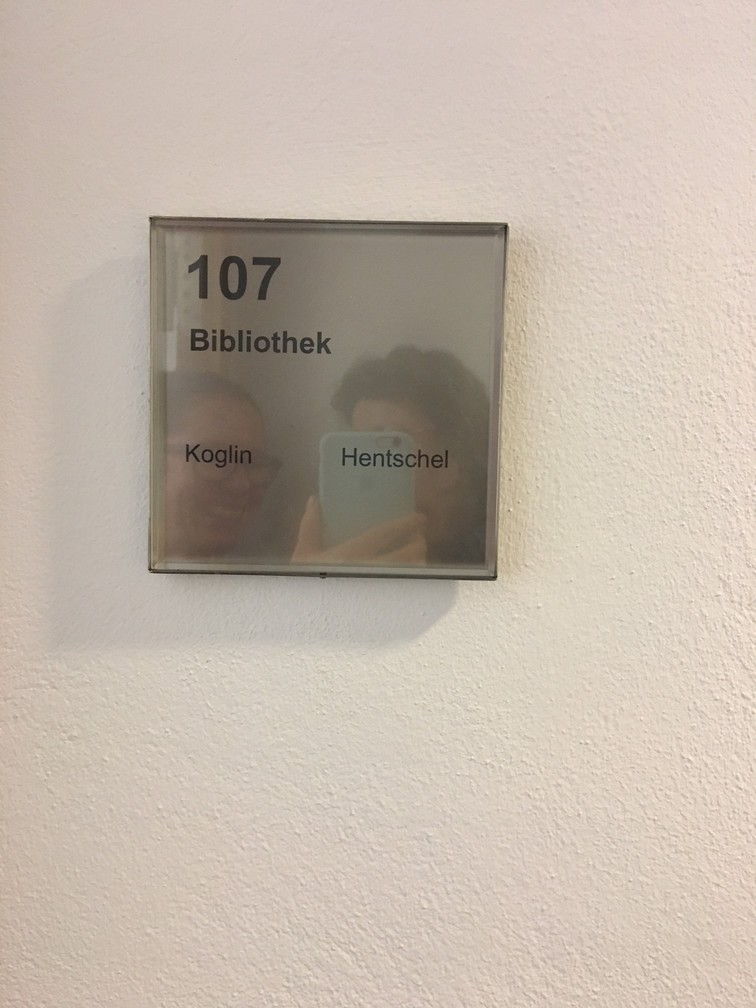
\includegraphics{igb/img/bibliothek.jpg}
\end{center}

Meine Kolleginnen. Wir sind eine Two-Persons-Library mit Hilfskraft und
ich habe einen sehr großen Respekt für Kolleginnen aus OPLs, die alles
alleine stemmen.

\hypertarget{was-stuxf6rt-sie-an-ihrer-bibliothek-beziehungsweise-was-wuxfcrden-sie-gerne-verbessern-wieso-stuxf6rt-sie-das-jetzt-noch}{%
\subsubsection*{Was stört Sie an Ihrer Bibliothek beziehungsweise was würden
Sie gerne verbessern? Wieso stört Sie das jetzt
(noch)?}\label{was-stuxf6rt-sie-an-ihrer-bibliothek-beziehungsweise-was-wuxfcrden-sie-gerne-verbessern-wieso-stuxf6rt-sie-das-jetzt-noch}}

\begin{center}
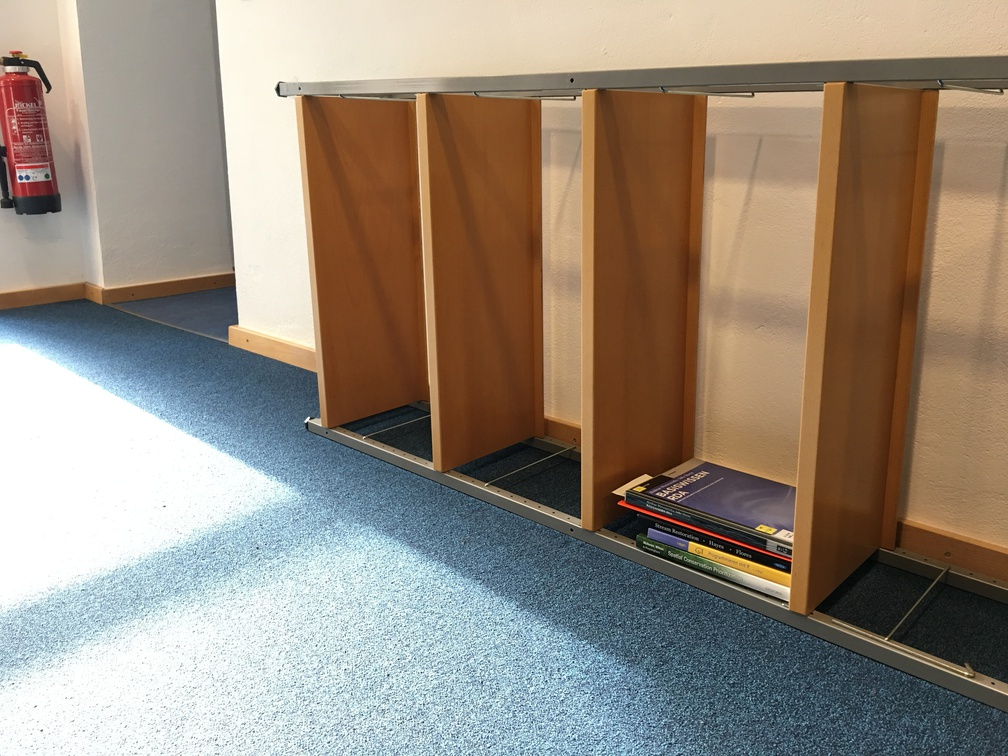
\includegraphics{igb/img/regal.jpg}
\end{center}

Wir sind gerade bei einem Projekt, bei dem wir mehrere tausend Bücher
umstellen. Physische Medien sind in ihrer Verwaltung, Bearbeitung und
täglichen Handhabung sehr aufwendig. Irgendwann dachte ich mal -- in den
Anfangsjahren der bibliothekarischen Tätigkeit -- so ein Regal ist
schnell umgeräumt oder ein paar Bücher schnell neu signiert. But, boy,
was I wrong\ldots{}

\hypertarget{zeigen-sie-uns-spuren-der-bibliotheksnutzung.-gibt-es-dazu-eine-geschichte}{%
\subsubsection*{Zeigen Sie uns Spuren der Bibliotheksnutzung. Gibt es dazu eine
Geschichte?}\label{zeigen-sie-uns-spuren-der-bibliotheksnutzung.-gibt-es-dazu-eine-geschichte}}

\begin{center}
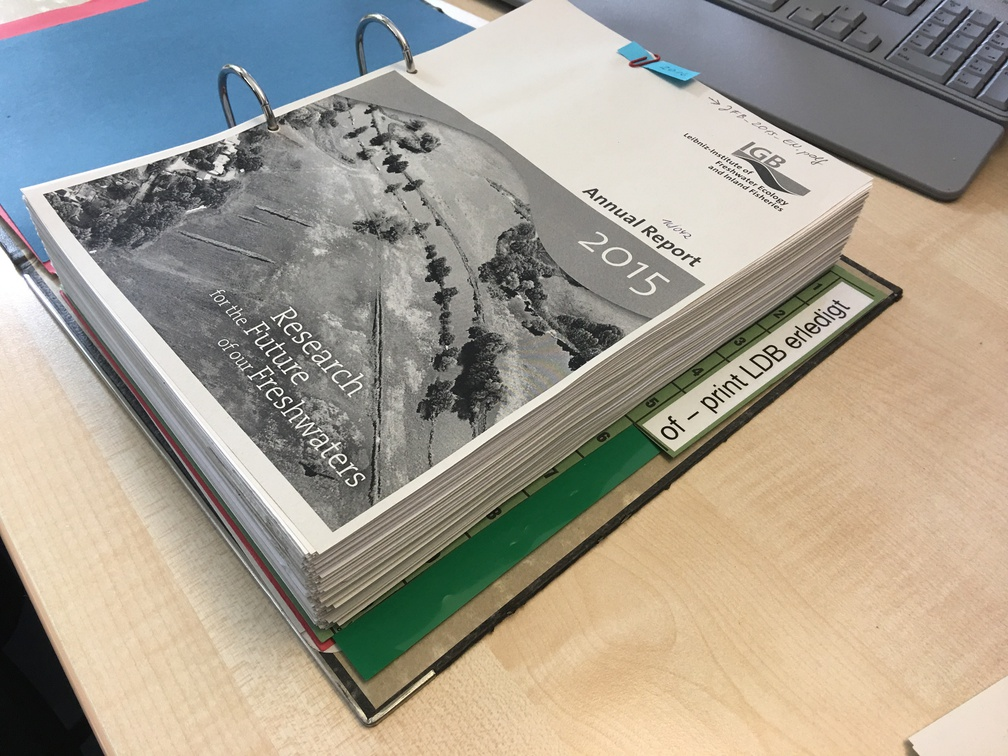
\includegraphics{igb/img/publikationen.jpg}
\end{center}

Auf dem Foto sieht man die ausgedruckten Titelseiten aller am Institut
erstellten Publikationen im Jahr 2016. Ich sehe sie auch als ein
Ergebnis der von Bibliotheken bereitgestellten gemeinsamen und lokalen
Infrastrukturen, ohne die Forschung nicht möglich wäre und die hier
wieder zurück in die Bibliothek finden.

\hypertarget{was-haben-sie-was-die-anderen-nicht-haben-warum-haben-sie-das-sollten-andere-es-auch-in-ihren-bibliotheken-haben}{%
\subsubsection*{Was haben Sie, was die anderen nicht haben? Warum haben Sie
das? Sollten andere es auch in ihren Bibliotheken
haben?}\label{was-haben-sie-was-die-anderen-nicht-haben-warum-haben-sie-das-sollten-andere-es-auch-in-ihren-bibliotheken-haben}}

\begin{center}
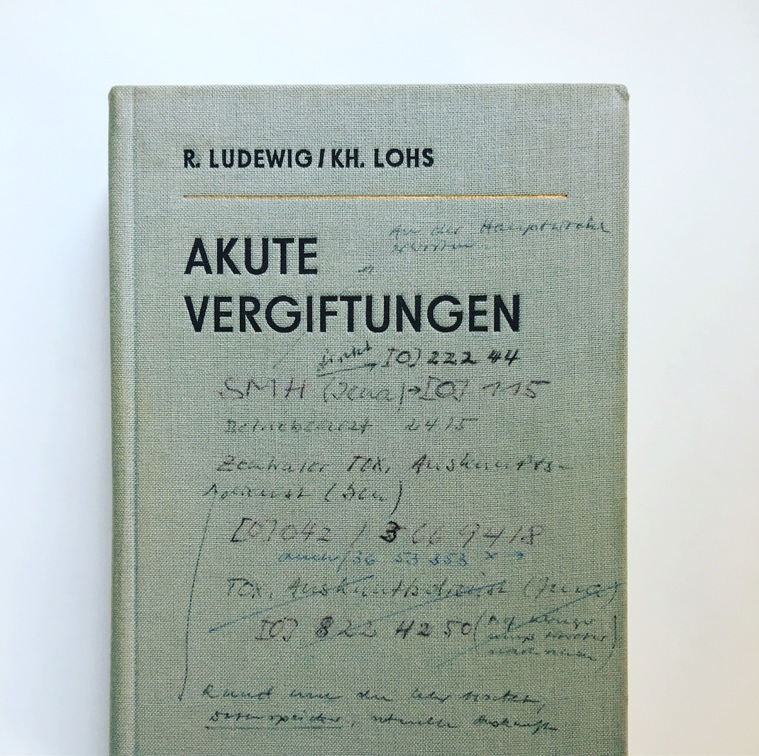
\includegraphics{igb/img/vergiftungen.jpg}
\end{center}

Auch wenn es das absolute No-Go ist, muss ich zugeben: Ich bin ein Fan
von Benutzungsspuren. Dieses Buch haben wir zufällig bei der
Bestandsdurchsicht gefunden. Elektronische Medien, für die wir heute den
Großteil unseres Budgets ausgeben, haben diese Spuren nicht. Bei allen
Vorteilen, die digitale Medien haben, vermisse ich es ein wenig, dass
Dateien niemals Geschichten erzählen werden können.

\hypertarget{ihre-bibliothek-name-adresse-spezialisierung-was-man-noch-uxfcber-sie-wissen-sollte}{%
\subsubsection*{Ihre Bibliothek (Name, Adresse, Spezialisierung, was man noch
über sie wissen
sollte)?}\label{ihre-bibliothek-name-adresse-spezialisierung-was-man-noch-uxfcber-sie-wissen-sollte}}

Bibliothek des Leibniz-Instituts für Gewässerökologie und
Binnenfischerei (IGB) im Forschungsverbund Berlin e.\,V., am Nordufer des
Müggelsees in Berlin-Friedrichshagen.

%autor
\begin{center}\rule{0.5\linewidth}{\linethickness}\end{center}

\textbf{Lydia Koglin}, nach geisteswissenschaftlichem Studium und
bibliothekswissenschaftlicher Ausbildung an einer Universitätsbibliothek
jetzt Leiterin einer Two-and-half-Woman-Bibliothek eines
umweltwissenschaftlichen Forschungsinstituts.
% !TEX root = ../master.tex

\vspace*{.5cm}
\section{Bibliothek des Leibniz-Instituts für Gewässerökologie und Binnenfischerei}
\begin{center}
\emph{Lydia Koglin}
\end{center}
\vspace*{1cm}

%body
\hypertarget{zeigen-sie-uns-den-ort-in-ihrer-bibliothek-an-dem-sie-die-meiste-zeit-verbringen.-was-ist-das-fuxfcr-ein-ort-wieso-sind-sie-die-meiste-zeit-dort}{%
\subsubsection*{Zeigen Sie uns den Ort in Ihrer Bibliothek, an dem Sie die
meiste Zeit verbringen. Was ist das für ein Ort? Wieso sind Sie die
meiste Zeit
dort?}\label{zeigen-sie-uns-den-ort-in-ihrer-bibliothek-an-dem-sie-die-meiste-zeit-verbringen.-was-ist-das-fuxfcr-ein-ort-wieso-sind-sie-die-meiste-zeit-dort}}

\begin{center}
\includegraphics{igb/img/internet.jpg}
\end{center}

Zweifelsohne verbringen wir die meiste Zeit irgendwo im Netz. Wenn das
Netz ausfällt -- was es glücklicherweise selten macht --, merkt man das
erst richtig. Gut, dass es dann noch ein paar Bücherregale gibt, in
denen man mal wieder Ordnung schaffen kann.

\hypertarget{was-wuxfcrden-sie-vermissen-wenn-es-nicht-mehr-da-wuxe4re-wieso-wuxfcrden-sie-es-vermissen}{%
\subsubsection*{Was würden Sie vermissen, wenn es nicht mehr da wäre? Wieso
würden Sie es
vermissen?}\label{was-wuxfcrden-sie-vermissen-wenn-es-nicht-mehr-da-wuxe4re-wieso-wuxfcrden-sie-es-vermissen}}

\begin{center}
\includegraphics{igb/img/bibliothek.jpg}
\end{center}

Meine Kolleginnen. Wir sind eine Two-Persons-Library mit Hilfskraft und
ich habe einen sehr großen Respekt für Kolleginnen aus OPLs, die alles
alleine stemmen.

\hypertarget{was-stuxf6rt-sie-an-ihrer-bibliothek-beziehungsweise-was-wuxfcrden-sie-gerne-verbessern-wieso-stuxf6rt-sie-das-jetzt-noch}{%
\subsubsection*{Was stört Sie an Ihrer Bibliothek beziehungsweise was würden
Sie gerne verbessern? Wieso stört Sie das jetzt
(noch)?}\label{was-stuxf6rt-sie-an-ihrer-bibliothek-beziehungsweise-was-wuxfcrden-sie-gerne-verbessern-wieso-stuxf6rt-sie-das-jetzt-noch}}

\begin{center}
\includegraphics{igb/img/regal.jpg}
\end{center}

Wir sind gerade bei einem Projekt, bei dem wir mehrere tausend Bücher
umstellen. Physische Medien sind in ihrer Verwaltung, Bearbeitung und
täglichen Handhabung sehr aufwendig. Irgendwann dachte ich mal -- in den
Anfangsjahren der bibliothekarischen Tätigkeit -- so ein Regal ist
schnell umgeräumt oder ein paar Bücher schnell neu signiert. But, boy,
was I wrong\ldots{}

\hypertarget{zeigen-sie-uns-spuren-der-bibliotheksnutzung.-gibt-es-dazu-eine-geschichte}{%
\subsubsection*{Zeigen Sie uns Spuren der Bibliotheksnutzung. Gibt es dazu eine
Geschichte?}\label{zeigen-sie-uns-spuren-der-bibliotheksnutzung.-gibt-es-dazu-eine-geschichte}}

\begin{center}
\includegraphics{igb/img/publikationen.jpg}
\end{center}

Auf dem Foto sieht man die ausgedruckten Titelseiten aller am Institut
erstellten Publikationen im Jahr 2016. Ich sehe sie auch als ein
Ergebnis der von Bibliotheken bereitgestellten gemeinsamen und lokalen
Infrastrukturen, ohne die Forschung nicht möglich wäre und die hier
wieder zurück in die Bibliothek finden.

\hypertarget{was-haben-sie-was-die-anderen-nicht-haben-warum-haben-sie-das-sollten-andere-es-auch-in-ihren-bibliotheken-haben}{%
\subsubsection*{Was haben Sie, was die anderen nicht haben? Warum haben Sie
das? Sollten andere es auch in ihren Bibliotheken
haben?}\label{was-haben-sie-was-die-anderen-nicht-haben-warum-haben-sie-das-sollten-andere-es-auch-in-ihren-bibliotheken-haben}}

\begin{center}
\includegraphics{igb/img/vergiftungen.jpg}
\end{center}

Auch wenn es das absolute No-Go ist, muss ich zugeben: Ich bin ein Fan
von Benutzungsspuren. Dieses Buch haben wir zufällig bei der
Bestandsdurchsicht gefunden. Elektronische Medien, für die wir heute den
Großteil unseres Budgets ausgeben, haben diese Spuren nicht. Bei allen
Vorteilen, die digitale Medien haben, vermisse ich es ein wenig, dass
Dateien niemals Geschichten erzählen werden können.

\hypertarget{ihre-bibliothek-name-adresse-spezialisierung-was-man-noch-uxfcber-sie-wissen-sollte}{%
\subsubsection*{Ihre Bibliothek (Name, Adresse, Spezialisierung, was man noch
über sie wissen
sollte)?}\label{ihre-bibliothek-name-adresse-spezialisierung-was-man-noch-uxfcber-sie-wissen-sollte}}

Bibliothek des Leibniz-Instituts für Gewässerökologie und
Binnenfischerei (IGB) im Forschungsverbund Berlin e.\,V., am Nordufer des
Müggelsees in Berlin-Friedrichshagen.

%autor
\begin{center}\rule{0.5\linewidth}{\linethickness}\end{center}

\textbf{Lydia Koglin}, nach geisteswissenschaftlichem Studium und
bibliothekswissenschaftlicher Ausbildung an einer Universitätsbibliothek
jetzt Leiterin einer Two-and-half-Woman-Bibliothek eines
umweltwissenschaftlichen Forschungsinstituts.
% !TEX root = ../master.tex

\vspace*{.5cm}
\section{Bibliothek des Leibniz-Instituts für Gewässerökologie und Binnenfischerei}
\begin{center}
\emph{Lydia Koglin}
\end{center}
\vspace*{1cm}

%body
\hypertarget{zeigen-sie-uns-den-ort-in-ihrer-bibliothek-an-dem-sie-die-meiste-zeit-verbringen.-was-ist-das-fuxfcr-ein-ort-wieso-sind-sie-die-meiste-zeit-dort}{%
\subsubsection*{Zeigen Sie uns den Ort in Ihrer Bibliothek, an dem Sie die
meiste Zeit verbringen. Was ist das für ein Ort? Wieso sind Sie die
meiste Zeit
dort?}\label{zeigen-sie-uns-den-ort-in-ihrer-bibliothek-an-dem-sie-die-meiste-zeit-verbringen.-was-ist-das-fuxfcr-ein-ort-wieso-sind-sie-die-meiste-zeit-dort}}

\begin{center}
\includegraphics{igb/img/internet.jpg}
\end{center}

Zweifelsohne verbringen wir die meiste Zeit irgendwo im Netz. Wenn das
Netz ausfällt -- was es glücklicherweise selten macht --, merkt man das
erst richtig. Gut, dass es dann noch ein paar Bücherregale gibt, in
denen man mal wieder Ordnung schaffen kann.

\hypertarget{was-wuxfcrden-sie-vermissen-wenn-es-nicht-mehr-da-wuxe4re-wieso-wuxfcrden-sie-es-vermissen}{%
\subsubsection*{Was würden Sie vermissen, wenn es nicht mehr da wäre? Wieso
würden Sie es
vermissen?}\label{was-wuxfcrden-sie-vermissen-wenn-es-nicht-mehr-da-wuxe4re-wieso-wuxfcrden-sie-es-vermissen}}

\begin{center}
\includegraphics{igb/img/bibliothek.jpg}
\end{center}

Meine Kolleginnen. Wir sind eine Two-Persons-Library mit Hilfskraft und
ich habe einen sehr großen Respekt für Kolleginnen aus OPLs, die alles
alleine stemmen.

\hypertarget{was-stuxf6rt-sie-an-ihrer-bibliothek-beziehungsweise-was-wuxfcrden-sie-gerne-verbessern-wieso-stuxf6rt-sie-das-jetzt-noch}{%
\subsubsection*{Was stört Sie an Ihrer Bibliothek beziehungsweise was würden
Sie gerne verbessern? Wieso stört Sie das jetzt
(noch)?}\label{was-stuxf6rt-sie-an-ihrer-bibliothek-beziehungsweise-was-wuxfcrden-sie-gerne-verbessern-wieso-stuxf6rt-sie-das-jetzt-noch}}

\begin{center}
\includegraphics{igb/img/regal.jpg}
\end{center}

Wir sind gerade bei einem Projekt, bei dem wir mehrere tausend Bücher
umstellen. Physische Medien sind in ihrer Verwaltung, Bearbeitung und
täglichen Handhabung sehr aufwendig. Irgendwann dachte ich mal -- in den
Anfangsjahren der bibliothekarischen Tätigkeit -- so ein Regal ist
schnell umgeräumt oder ein paar Bücher schnell neu signiert. But, boy,
was I wrong\ldots{}

\hypertarget{zeigen-sie-uns-spuren-der-bibliotheksnutzung.-gibt-es-dazu-eine-geschichte}{%
\subsubsection*{Zeigen Sie uns Spuren der Bibliotheksnutzung. Gibt es dazu eine
Geschichte?}\label{zeigen-sie-uns-spuren-der-bibliotheksnutzung.-gibt-es-dazu-eine-geschichte}}

\begin{center}
\includegraphics{igb/img/publikationen.jpg}
\end{center}

Auf dem Foto sieht man die ausgedruckten Titelseiten aller am Institut
erstellten Publikationen im Jahr 2016. Ich sehe sie auch als ein
Ergebnis der von Bibliotheken bereitgestellten gemeinsamen und lokalen
Infrastrukturen, ohne die Forschung nicht möglich wäre und die hier
wieder zurück in die Bibliothek finden.

\hypertarget{was-haben-sie-was-die-anderen-nicht-haben-warum-haben-sie-das-sollten-andere-es-auch-in-ihren-bibliotheken-haben}{%
\subsubsection*{Was haben Sie, was die anderen nicht haben? Warum haben Sie
das? Sollten andere es auch in ihren Bibliotheken
haben?}\label{was-haben-sie-was-die-anderen-nicht-haben-warum-haben-sie-das-sollten-andere-es-auch-in-ihren-bibliotheken-haben}}

\begin{center}
\includegraphics{igb/img/vergiftungen.jpg}
\end{center}

Auch wenn es das absolute No-Go ist, muss ich zugeben: Ich bin ein Fan
von Benutzungsspuren. Dieses Buch haben wir zufällig bei der
Bestandsdurchsicht gefunden. Elektronische Medien, für die wir heute den
Großteil unseres Budgets ausgeben, haben diese Spuren nicht. Bei allen
Vorteilen, die digitale Medien haben, vermisse ich es ein wenig, dass
Dateien niemals Geschichten erzählen werden können.

\hypertarget{ihre-bibliothek-name-adresse-spezialisierung-was-man-noch-uxfcber-sie-wissen-sollte}{%
\subsubsection*{Ihre Bibliothek (Name, Adresse, Spezialisierung, was man noch
über sie wissen
sollte)?}\label{ihre-bibliothek-name-adresse-spezialisierung-was-man-noch-uxfcber-sie-wissen-sollte}}

Bibliothek des Leibniz-Instituts für Gewässerökologie und
Binnenfischerei (IGB) im Forschungsverbund Berlin e.\,V., am Nordufer des
Müggelsees in Berlin-Friedrichshagen.

%autor
\begin{center}\rule{0.5\linewidth}{\linethickness}\end{center}

\textbf{Lydia Koglin}, nach geisteswissenschaftlichem Studium und
bibliothekswissenschaftlicher Ausbildung an einer Universitätsbibliothek
jetzt Leiterin einer Two-and-half-Woman-Bibliothek eines
umweltwissenschaftlichen Forschungsinstituts.
% !TEX root = ../master.tex

\vspace*{.5cm}
\section{Bibliothek des Leibniz-Instituts für Gewässerökologie und Binnenfischerei}
\begin{center}
\emph{Lydia Koglin}
\end{center}
\vspace*{1cm}

%body
\hypertarget{zeigen-sie-uns-den-ort-in-ihrer-bibliothek-an-dem-sie-die-meiste-zeit-verbringen.-was-ist-das-fuxfcr-ein-ort-wieso-sind-sie-die-meiste-zeit-dort}{%
\subsubsection*{Zeigen Sie uns den Ort in Ihrer Bibliothek, an dem Sie die
meiste Zeit verbringen. Was ist das für ein Ort? Wieso sind Sie die
meiste Zeit
dort?}\label{zeigen-sie-uns-den-ort-in-ihrer-bibliothek-an-dem-sie-die-meiste-zeit-verbringen.-was-ist-das-fuxfcr-ein-ort-wieso-sind-sie-die-meiste-zeit-dort}}

\begin{center}
\includegraphics{igb/img/internet.jpg}
\end{center}

Zweifelsohne verbringen wir die meiste Zeit irgendwo im Netz. Wenn das
Netz ausfällt -- was es glücklicherweise selten macht --, merkt man das
erst richtig. Gut, dass es dann noch ein paar Bücherregale gibt, in
denen man mal wieder Ordnung schaffen kann.

\hypertarget{was-wuxfcrden-sie-vermissen-wenn-es-nicht-mehr-da-wuxe4re-wieso-wuxfcrden-sie-es-vermissen}{%
\subsubsection*{Was würden Sie vermissen, wenn es nicht mehr da wäre? Wieso
würden Sie es
vermissen?}\label{was-wuxfcrden-sie-vermissen-wenn-es-nicht-mehr-da-wuxe4re-wieso-wuxfcrden-sie-es-vermissen}}

\begin{center}
\includegraphics{igb/img/bibliothek.jpg}
\end{center}

Meine Kolleginnen. Wir sind eine Two-Persons-Library mit Hilfskraft und
ich habe einen sehr großen Respekt für Kolleginnen aus OPLs, die alles
alleine stemmen.

\hypertarget{was-stuxf6rt-sie-an-ihrer-bibliothek-beziehungsweise-was-wuxfcrden-sie-gerne-verbessern-wieso-stuxf6rt-sie-das-jetzt-noch}{%
\subsubsection*{Was stört Sie an Ihrer Bibliothek beziehungsweise was würden
Sie gerne verbessern? Wieso stört Sie das jetzt
(noch)?}\label{was-stuxf6rt-sie-an-ihrer-bibliothek-beziehungsweise-was-wuxfcrden-sie-gerne-verbessern-wieso-stuxf6rt-sie-das-jetzt-noch}}

\begin{center}
\includegraphics{igb/img/regal.jpg}
\end{center}

Wir sind gerade bei einem Projekt, bei dem wir mehrere tausend Bücher
umstellen. Physische Medien sind in ihrer Verwaltung, Bearbeitung und
täglichen Handhabung sehr aufwendig. Irgendwann dachte ich mal -- in den
Anfangsjahren der bibliothekarischen Tätigkeit -- so ein Regal ist
schnell umgeräumt oder ein paar Bücher schnell neu signiert. But, boy,
was I wrong\ldots{}

\hypertarget{zeigen-sie-uns-spuren-der-bibliotheksnutzung.-gibt-es-dazu-eine-geschichte}{%
\subsubsection*{Zeigen Sie uns Spuren der Bibliotheksnutzung. Gibt es dazu eine
Geschichte?}\label{zeigen-sie-uns-spuren-der-bibliotheksnutzung.-gibt-es-dazu-eine-geschichte}}

\begin{center}
\includegraphics{igb/img/publikationen.jpg}
\end{center}

Auf dem Foto sieht man die ausgedruckten Titelseiten aller am Institut
erstellten Publikationen im Jahr 2016. Ich sehe sie auch als ein
Ergebnis der von Bibliotheken bereitgestellten gemeinsamen und lokalen
Infrastrukturen, ohne die Forschung nicht möglich wäre und die hier
wieder zurück in die Bibliothek finden.

\hypertarget{was-haben-sie-was-die-anderen-nicht-haben-warum-haben-sie-das-sollten-andere-es-auch-in-ihren-bibliotheken-haben}{%
\subsubsection*{Was haben Sie, was die anderen nicht haben? Warum haben Sie
das? Sollten andere es auch in ihren Bibliotheken
haben?}\label{was-haben-sie-was-die-anderen-nicht-haben-warum-haben-sie-das-sollten-andere-es-auch-in-ihren-bibliotheken-haben}}

\begin{center}
\includegraphics{igb/img/vergiftungen.jpg}
\end{center}

Auch wenn es das absolute No-Go ist, muss ich zugeben: Ich bin ein Fan
von Benutzungsspuren. Dieses Buch haben wir zufällig bei der
Bestandsdurchsicht gefunden. Elektronische Medien, für die wir heute den
Großteil unseres Budgets ausgeben, haben diese Spuren nicht. Bei allen
Vorteilen, die digitale Medien haben, vermisse ich es ein wenig, dass
Dateien niemals Geschichten erzählen werden können.

\hypertarget{ihre-bibliothek-name-adresse-spezialisierung-was-man-noch-uxfcber-sie-wissen-sollte}{%
\subsubsection*{Ihre Bibliothek (Name, Adresse, Spezialisierung, was man noch
über sie wissen
sollte)?}\label{ihre-bibliothek-name-adresse-spezialisierung-was-man-noch-uxfcber-sie-wissen-sollte}}

Bibliothek des Leibniz-Instituts für Gewässerökologie und
Binnenfischerei (IGB) im Forschungsverbund Berlin e.\,V., am Nordufer des
Müggelsees in Berlin-Friedrichshagen.

%autor
\begin{center}\rule{0.5\linewidth}{\linethickness}\end{center}

\textbf{Lydia Koglin}, nach geisteswissenschaftlichem Studium und
bibliothekswissenschaftlicher Ausbildung an einer Universitätsbibliothek
jetzt Leiterin einer Two-and-half-Woman-Bibliothek eines
umweltwissenschaftlichen Forschungsinstituts.
% !TEX root = ../master.tex

\vspace*{.5cm}
\section{Bibliothek des Leibniz-Instituts für Gewässerökologie und Binnenfischerei}
\begin{center}
\emph{Lydia Koglin}
\end{center}
\vspace*{1cm}

%body
\hypertarget{zeigen-sie-uns-den-ort-in-ihrer-bibliothek-an-dem-sie-die-meiste-zeit-verbringen.-was-ist-das-fuxfcr-ein-ort-wieso-sind-sie-die-meiste-zeit-dort}{%
\subsubsection*{Zeigen Sie uns den Ort in Ihrer Bibliothek, an dem Sie die
meiste Zeit verbringen. Was ist das für ein Ort? Wieso sind Sie die
meiste Zeit
dort?}\label{zeigen-sie-uns-den-ort-in-ihrer-bibliothek-an-dem-sie-die-meiste-zeit-verbringen.-was-ist-das-fuxfcr-ein-ort-wieso-sind-sie-die-meiste-zeit-dort}}

\begin{center}
\includegraphics{igb/img/internet.jpg}
\end{center}

Zweifelsohne verbringen wir die meiste Zeit irgendwo im Netz. Wenn das
Netz ausfällt -- was es glücklicherweise selten macht --, merkt man das
erst richtig. Gut, dass es dann noch ein paar Bücherregale gibt, in
denen man mal wieder Ordnung schaffen kann.

\hypertarget{was-wuxfcrden-sie-vermissen-wenn-es-nicht-mehr-da-wuxe4re-wieso-wuxfcrden-sie-es-vermissen}{%
\subsubsection*{Was würden Sie vermissen, wenn es nicht mehr da wäre? Wieso
würden Sie es
vermissen?}\label{was-wuxfcrden-sie-vermissen-wenn-es-nicht-mehr-da-wuxe4re-wieso-wuxfcrden-sie-es-vermissen}}

\begin{center}
\includegraphics{igb/img/bibliothek.jpg}
\end{center}

Meine Kolleginnen. Wir sind eine Two-Persons-Library mit Hilfskraft und
ich habe einen sehr großen Respekt für Kolleginnen aus OPLs, die alles
alleine stemmen.

\hypertarget{was-stuxf6rt-sie-an-ihrer-bibliothek-beziehungsweise-was-wuxfcrden-sie-gerne-verbessern-wieso-stuxf6rt-sie-das-jetzt-noch}{%
\subsubsection*{Was stört Sie an Ihrer Bibliothek beziehungsweise was würden
Sie gerne verbessern? Wieso stört Sie das jetzt
(noch)?}\label{was-stuxf6rt-sie-an-ihrer-bibliothek-beziehungsweise-was-wuxfcrden-sie-gerne-verbessern-wieso-stuxf6rt-sie-das-jetzt-noch}}

\begin{center}
\includegraphics{igb/img/regal.jpg}
\end{center}

Wir sind gerade bei einem Projekt, bei dem wir mehrere tausend Bücher
umstellen. Physische Medien sind in ihrer Verwaltung, Bearbeitung und
täglichen Handhabung sehr aufwendig. Irgendwann dachte ich mal -- in den
Anfangsjahren der bibliothekarischen Tätigkeit -- so ein Regal ist
schnell umgeräumt oder ein paar Bücher schnell neu signiert. But, boy,
was I wrong\ldots{}

\hypertarget{zeigen-sie-uns-spuren-der-bibliotheksnutzung.-gibt-es-dazu-eine-geschichte}{%
\subsubsection*{Zeigen Sie uns Spuren der Bibliotheksnutzung. Gibt es dazu eine
Geschichte?}\label{zeigen-sie-uns-spuren-der-bibliotheksnutzung.-gibt-es-dazu-eine-geschichte}}

\begin{center}
\includegraphics{igb/img/publikationen.jpg}
\end{center}

Auf dem Foto sieht man die ausgedruckten Titelseiten aller am Institut
erstellten Publikationen im Jahr 2016. Ich sehe sie auch als ein
Ergebnis der von Bibliotheken bereitgestellten gemeinsamen und lokalen
Infrastrukturen, ohne die Forschung nicht möglich wäre und die hier
wieder zurück in die Bibliothek finden.

\hypertarget{was-haben-sie-was-die-anderen-nicht-haben-warum-haben-sie-das-sollten-andere-es-auch-in-ihren-bibliotheken-haben}{%
\subsubsection*{Was haben Sie, was die anderen nicht haben? Warum haben Sie
das? Sollten andere es auch in ihren Bibliotheken
haben?}\label{was-haben-sie-was-die-anderen-nicht-haben-warum-haben-sie-das-sollten-andere-es-auch-in-ihren-bibliotheken-haben}}

\begin{center}
\includegraphics{igb/img/vergiftungen.jpg}
\end{center}

Auch wenn es das absolute No-Go ist, muss ich zugeben: Ich bin ein Fan
von Benutzungsspuren. Dieses Buch haben wir zufällig bei der
Bestandsdurchsicht gefunden. Elektronische Medien, für die wir heute den
Großteil unseres Budgets ausgeben, haben diese Spuren nicht. Bei allen
Vorteilen, die digitale Medien haben, vermisse ich es ein wenig, dass
Dateien niemals Geschichten erzählen werden können.

\hypertarget{ihre-bibliothek-name-adresse-spezialisierung-was-man-noch-uxfcber-sie-wissen-sollte}{%
\subsubsection*{Ihre Bibliothek (Name, Adresse, Spezialisierung, was man noch
über sie wissen
sollte)?}\label{ihre-bibliothek-name-adresse-spezialisierung-was-man-noch-uxfcber-sie-wissen-sollte}}

Bibliothek des Leibniz-Instituts für Gewässerökologie und
Binnenfischerei (IGB) im Forschungsverbund Berlin e.\,V., am Nordufer des
Müggelsees in Berlin-Friedrichshagen.

%autor
\begin{center}\rule{0.5\linewidth}{\linethickness}\end{center}

\textbf{Lydia Koglin}, nach geisteswissenschaftlichem Studium und
bibliothekswissenschaftlicher Ausbildung an einer Universitätsbibliothek
jetzt Leiterin einer Two-and-half-Woman-Bibliothek eines
umweltwissenschaftlichen Forschungsinstituts.
% !TEX root = ../master.tex

\vspace*{.5cm}
\section{Bibliothek des Leibniz-Instituts für Gewässerökologie und Binnenfischerei}
\begin{center}
\emph{Lydia Koglin}
\end{center}
\vspace*{1cm}

%body
\hypertarget{zeigen-sie-uns-den-ort-in-ihrer-bibliothek-an-dem-sie-die-meiste-zeit-verbringen.-was-ist-das-fuxfcr-ein-ort-wieso-sind-sie-die-meiste-zeit-dort}{%
\subsubsection*{Zeigen Sie uns den Ort in Ihrer Bibliothek, an dem Sie die
meiste Zeit verbringen. Was ist das für ein Ort? Wieso sind Sie die
meiste Zeit
dort?}\label{zeigen-sie-uns-den-ort-in-ihrer-bibliothek-an-dem-sie-die-meiste-zeit-verbringen.-was-ist-das-fuxfcr-ein-ort-wieso-sind-sie-die-meiste-zeit-dort}}

\begin{center}
\includegraphics{igb/img/internet.jpg}
\end{center}

Zweifelsohne verbringen wir die meiste Zeit irgendwo im Netz. Wenn das
Netz ausfällt -- was es glücklicherweise selten macht --, merkt man das
erst richtig. Gut, dass es dann noch ein paar Bücherregale gibt, in
denen man mal wieder Ordnung schaffen kann.

\hypertarget{was-wuxfcrden-sie-vermissen-wenn-es-nicht-mehr-da-wuxe4re-wieso-wuxfcrden-sie-es-vermissen}{%
\subsubsection*{Was würden Sie vermissen, wenn es nicht mehr da wäre? Wieso
würden Sie es
vermissen?}\label{was-wuxfcrden-sie-vermissen-wenn-es-nicht-mehr-da-wuxe4re-wieso-wuxfcrden-sie-es-vermissen}}

\begin{center}
\includegraphics{igb/img/bibliothek.jpg}
\end{center}

Meine Kolleginnen. Wir sind eine Two-Persons-Library mit Hilfskraft und
ich habe einen sehr großen Respekt für Kolleginnen aus OPLs, die alles
alleine stemmen.

\hypertarget{was-stuxf6rt-sie-an-ihrer-bibliothek-beziehungsweise-was-wuxfcrden-sie-gerne-verbessern-wieso-stuxf6rt-sie-das-jetzt-noch}{%
\subsubsection*{Was stört Sie an Ihrer Bibliothek beziehungsweise was würden
Sie gerne verbessern? Wieso stört Sie das jetzt
(noch)?}\label{was-stuxf6rt-sie-an-ihrer-bibliothek-beziehungsweise-was-wuxfcrden-sie-gerne-verbessern-wieso-stuxf6rt-sie-das-jetzt-noch}}

\begin{center}
\includegraphics{igb/img/regal.jpg}
\end{center}

Wir sind gerade bei einem Projekt, bei dem wir mehrere tausend Bücher
umstellen. Physische Medien sind in ihrer Verwaltung, Bearbeitung und
täglichen Handhabung sehr aufwendig. Irgendwann dachte ich mal -- in den
Anfangsjahren der bibliothekarischen Tätigkeit -- so ein Regal ist
schnell umgeräumt oder ein paar Bücher schnell neu signiert. But, boy,
was I wrong\ldots{}

\hypertarget{zeigen-sie-uns-spuren-der-bibliotheksnutzung.-gibt-es-dazu-eine-geschichte}{%
\subsubsection*{Zeigen Sie uns Spuren der Bibliotheksnutzung. Gibt es dazu eine
Geschichte?}\label{zeigen-sie-uns-spuren-der-bibliotheksnutzung.-gibt-es-dazu-eine-geschichte}}

\begin{center}
\includegraphics{igb/img/publikationen.jpg}
\end{center}

Auf dem Foto sieht man die ausgedruckten Titelseiten aller am Institut
erstellten Publikationen im Jahr 2016. Ich sehe sie auch als ein
Ergebnis der von Bibliotheken bereitgestellten gemeinsamen und lokalen
Infrastrukturen, ohne die Forschung nicht möglich wäre und die hier
wieder zurück in die Bibliothek finden.

\hypertarget{was-haben-sie-was-die-anderen-nicht-haben-warum-haben-sie-das-sollten-andere-es-auch-in-ihren-bibliotheken-haben}{%
\subsubsection*{Was haben Sie, was die anderen nicht haben? Warum haben Sie
das? Sollten andere es auch in ihren Bibliotheken
haben?}\label{was-haben-sie-was-die-anderen-nicht-haben-warum-haben-sie-das-sollten-andere-es-auch-in-ihren-bibliotheken-haben}}

\begin{center}
\includegraphics{igb/img/vergiftungen.jpg}
\end{center}

Auch wenn es das absolute No-Go ist, muss ich zugeben: Ich bin ein Fan
von Benutzungsspuren. Dieses Buch haben wir zufällig bei der
Bestandsdurchsicht gefunden. Elektronische Medien, für die wir heute den
Großteil unseres Budgets ausgeben, haben diese Spuren nicht. Bei allen
Vorteilen, die digitale Medien haben, vermisse ich es ein wenig, dass
Dateien niemals Geschichten erzählen werden können.

\hypertarget{ihre-bibliothek-name-adresse-spezialisierung-was-man-noch-uxfcber-sie-wissen-sollte}{%
\subsubsection*{Ihre Bibliothek (Name, Adresse, Spezialisierung, was man noch
über sie wissen
sollte)?}\label{ihre-bibliothek-name-adresse-spezialisierung-was-man-noch-uxfcber-sie-wissen-sollte}}

Bibliothek des Leibniz-Instituts für Gewässerökologie und
Binnenfischerei (IGB) im Forschungsverbund Berlin e.\,V., am Nordufer des
Müggelsees in Berlin-Friedrichshagen.

%autor
\begin{center}\rule{0.5\linewidth}{\linethickness}\end{center}

\textbf{Lydia Koglin}, nach geisteswissenschaftlichem Studium und
bibliothekswissenschaftlicher Ausbildung an einer Universitätsbibliothek
jetzt Leiterin einer Two-and-half-Woman-Bibliothek eines
umweltwissenschaftlichen Forschungsinstituts.

\end{document}
